%% Copernicus Publications Manuscript Preparation Template for LaTeX Submissions
%% ---------------------------------
%% This template should be used for copernicus.cls
%% The class file and some style files are bundled in the Copernicus Latex Package, which can be downloaded from the different journal webpages.
%% For further assistance please contact Copernicus Publications at: production@copernicus.org
%% https://publications.copernicus.org/for_authors/manuscript_preparation.html


%% Please use the following documentclass and journal abbreviations for preprints and final revised papers.

%% 2-column papers and preprints
\documentclass[acp, manuscript]{copernicus}

\newcommand{\tcr}{\textcolor{red}}
\newcommand{\tcb}{\textcolor{blue}}

%% Journal abbreviations (please use the same for preprints and final revised papers)

\begin{document}

\title{A framework for understanding and narrowing uncertainties for Solar Radiation Modification modeling experiments}


% \Author[affil]{given_name}{surname}

\Author[1]{Daniele}{Visioni}
\Author[2]{Ben}{Kravitz}
\Author[3]{Douglas G.}{MacMartin}
\Author[4]{Timofei}{Sukodolov}
\Author[5]{Gabriel}{Chiodo}


\affil[1]{Department of Earth and Atmospheric Sciences, Cornell University, Ithaca, NY, 14850}
\affil[2]{Department of Earth and Atmospheric Sciences, Indiana University, Bloomington, IN, 47405}
\affil[3]{Sibley School of Mechanical and Aerospace Engineering, Cornell University, Ithaca, NY 14850, USA}
\affil[4]{Physikalisch-Meteorologisches Observatorium Davos/World Radiation Center, Davos, Switzerland}
\affil[5]{Instituto de Geociencias, CSIC, Madrid, 28040}
%\affil[]{ADDRESS}

%% The [] brackets identify the author with the corresponding affiliation. 1, 2, 3, etc. should be inserted.

%% If an author is deceased, please mark the respective author name(s) with a dagger, e.g. "\Author[2,$\dag$]{Anton}{Smith}", and add a further "\affil[$\dag$]{deceased, 1 July 2019}".

%% If authors contributed equally, please mark the respective author names with an asterisk, e.g. "\Author[2,*]{Anton}{Smith}" and "\Author[3,*]{Bradley}{Miller}" and add a further affiliation: "\affil[*]{These authors contributed equally to this work.}".


\correspondence{Daniele Visioni (dv224@cornell.edu)}

\runningtitle{TEXT}

\runningauthor{TEXT}





\received{}
\pubdiscuss{} %% only important for two-stage journals
\revised{}
\accepted{}
\published{}

%% These dates will be inserted by Copernicus Publications during the typesetting process.


\firstpage{1}

\maketitle



\begin{abstract}
Having a clear conceptualization of what constitutes an uncertainty, and what its sources might be in a specific field of investigation, is crucial to understanding which of the sources can be better constrained and how. For the topic of Solar Radiation Modification (SRM), this is particularly important as the scientific community, as well as countries and international bodies, grapple with the problem of deciding how (and if) to pursue research programs capable of narrowing its related uncertainties.
Here we discuss those uncertainties that can be investigated through the use of climate model simulations. We define as a useful metric for our concept of uncertainty as the spread in global, regional, or local projections for any given climate-relevant variable, given a set of simulations spanning different climate models and/or different scenarios.

We propose to separate this concept of uncertainty for the purpose of SRM evaluation into the following two macro-categories: the first is storyline uncertainty, which includes the sub-categories of scenario uncertainty (related to emissions and societal response); target uncertainty (what is the specific target that SRM tries to achieve) and strategy uncertainty (how is the SRM method deployed to achieve the target). The second is physical uncertainty, which can be investigated through the exploration of both inter-model SRM uncertainty (related to the Earth system processes specific to SRM) and inter-model climate uncertainty (related to underlying uncertainty in the representation of climatic processes). Finally, there is a component of internal variability that can be treated similarly to climate change.

We apply our framework to a large set of climate model simulations of stratospheric aerosol injections (SAI) and find four important results using our framework analyzing surface temperature and precipitation data: 1) in the same set of models, inter-model uncertainties due to an increase in temperatures of, on average, 2$^{\circ}$C are larger than inter-model uncertainties from SAI aimed at avoiding that increase, independently of spatial aggregation considered, (68\% larger for surface temperatures, 23\% larger for annual precipitation); 2) inter-model SRM uncertainties in SAI simulations are strongly driven by uncertainties in the differing simulation of aerosols and their transport, including their impacts on composition, circulation, and other secondary effects, leading us to conclude that resolving such uncertainties across different models has the potential to reduce overall uncertainties by over 61\% for surface temperatures and 64\% for precipitation; 3) uncertainties related to the deployment of different kind of aerosols in a single model are small compared to inter-model SRM uncertainties, constituting only a 9\% and 17\% portion of overall uncertainties, respectively, for surface temperatures and precipitation, with some important regional differences for the latter; 4) by looking at results of different strategies and scenarios with one single model, we conclude that, while at the global level temperature and precipitation are overwhelmingly driven by target uncertainty, at the regional level the strategy uncertainty can be a relevant portion of the overall storyline uncertainty. 

\end{abstract}



\introduction  %% \introduction[modified heading if necessary]

The concept of scientific uncertainty has long occupied a central place in the philosophy of science. The fundamental epistemological challenge, as outlined firstly by David Hume, is that no finite set of observations can justify universal claims about nature \citep{Rosenberg_1993}. In the 20th century, various philosophers expanded on this observation, which was intended as the evidence of a limitation of empirical knowledge, by establishing uncertainty as the defining feature of scientific inquiry, rather than a flaw: the fact that scientific theories can be falsified is a strength of the scientific process \citep{popper2005logic,lakatos1974popper,Slavov2018-SLAHTP}. \\

Climate science (and more specifically, climate models) exemplifies more than other fields the challenges and importance of conceptualizing scientific uncertainty \citep[see, for instance, the work of Elizabeth Lloyd, especially][]{Lloyd_2010}.  Climate models are indispensable tools for projecting future climate conditions, yet they are subject to multiple sources of uncertainty: the more familiar, simple categorization of such uncertainties include: i) structural uncertainty from model design, ii) parametric uncertainty from input values, iii) and scenario uncertainty from socio-economic assumptions  \citep{Hawkins2009,Lehner2020}. Various, more detailed and specific proposed frameworks to classify these uncertainties exist \citep{Frigg2015,BEVAN2022102919} , with the purpose to identify opportunities for further improvement, as well as to provide a basis for decision-making in the context of unresolvable uncertainties. It is also important to acknowledge, however, that such uncertainties - and the perception of the ``uncertainty'' of climate science - have been used as leverage to cast doubt on climate science as a whole \citep{LEWANDOWSKY20151}.
Considering scientific uncertainty in policy-relevant fields can’t be done without also including societal considerations. \citep{Douglas2009-DOUSPA-2} importantly argued that non-epistemic values—such as ethical, social, or political considerations—play a legitimate and often necessary role in scientific reasoning, especially when uncertainty is high and the consequences of error are significant.  In climate science, decisions about how much evidence is sufficient to warrant policy action cannot be made purely on epistemic grounds; they also depend on judgments about acceptable risk and societal priorities.\\

While this discussion has been happening for decades in the context of climate science in general \citep{Oreskes2004}, there is far more sparse literature when it comes to climate intervention methods, and Solar Radiation Modification (SRM) in particular. The idea itself is ``simple'' from a physical perspective: if climate change is a result of an energy imbalance, due to more greenhouse gases increasing Earth’s emissivity, such an imbalance might be reduced if incoming solar radiation is reduced through one or more methods that can help reflect some of it before it reaches the surface \citep{Budyko1977,Govin2003}. The apparent simplicity, however, belies an even more intricate ethical and sociopolitical landscape than for climate change. While plenty of emerging literature outlines the various ethical concerns related to SRM \citep[for a recent review, see][]{Flegal2019}, less has been said about how the conceptualization of scientific uncertainty in the SRM context has shaped discussions of SRM itself \citep[an exception being][]{Wiertz2016}.  To understand the importance of such framing, we can consider the difference between how scientific uncertainties are understood or perceived between climate change and SRM in relation to the Precautionary Principle (PP).  In one of its main formulations the PP states that ``Where there are threats of serious and irreversible damage, lack of scientific certainty shall not be used as a reason for postponing cost-effective measures to prevent environmental degradation'' (Article 15 of the 1992 Rio Declaration on Environment and Development, see \cite{Hopster2023} for a recent discussion of the PP in the context of climate uncertainty). Using this framework for climate change has usually been understood to mean that a lack of certainty over the impacts of global warming should not be an obstacle for emission reductions, and that further information over the severity of the impacts are needed to inform better adaptation practices, rather than to simply determine the urgency with which mitigation is required. For SRM however, due to the deliberate nature of the intervention, and to its fundamental design aspect \citep{Kravitz2016}, the application of the principle is more complicated, and can be applied in different ways \citep{Tedsen2013,Davies_Vinders_2025}, also depending on how the concept of uncertainty and its capacity to be reduced is treated: at the two extremes, one can argue that both the potential risks and uncertainties from SRM are too large (and unresolvable) to ever consider, while on the other, that the real risks of climate change are too large not to consider SRM \citep{Baiman2024}. In between these, there is space to consider if and how SRM uncertainties could be reduced through further research, and what kind of research, and how such a reduction could affect overall assessments of SRM risks and potential decisions around deployments.
In the following section, we will review some relevant examples from the scientific literature and international reports where SRM is discussed in the context of its uncertainties, as a starting point for the rest of our discussion.\\

\subsection{SRM and uncertainties in past literature and scientific assessments}

The natural place to start for such a review is the Intergovernmental Panel on Climate Change (IPCC) reports. The IPCC has over time developed its own framework for characterizing and communicating uncertainty, which it defines as ``a state of incomplete knowledge that can result from a lack of information or from disagreement about what is known or even knowable'' \citep{IPCC_2013_WGI_SPM}. As discussed in \cite{mastrandrea2011ipcc}, the IPCC refined its own language around uncertainty in order to characterize the findings of the assessment processes, namely around two complementary metrics: confidence, which synthesizes the type, amount, quality, and consistency of evidence and the degree of agreement among experts, and quantification of likelihood, which expresses quantified probabilities of outcomes based on statistical analysis or expert judgment.

The IPCC, in its Working Group III (Mitigation of Climate Change) Sixth Assessment Report \citep{IPCC_2022_WGIII}, mentions multiple times the presence of uncertainties related to Solar Radiation Modification (SRM). The most relevant excerpts are reported below (emphasis on the word uncertainty or similar words are ours):

\begin{enumerate}
    \item ``Solar radiation modification (SRM) could potentially cool the planet rapidly at low estimated direct costs by reflecting incoming sunlight, but entails uncertain side effects and thorny international equity and governance challenges [...]''
    \item ``Understanding the climate response to SRM remains subject to large uncertainties [...]''
    \item ``There also are significant uncertainties surrounding SRM, including uncertainties on the costs and risks, which can substantially alter the amount of SRM used in modelled pathways''
    \item ``[...] there is low confidence in understanding of the climate response to SRM at the regional scale [...]” “Nevertheless, large uncertainties still exist for climate processes associated with SRM options (e.g. aerosol-cloud radiation interaction)''
\end{enumerate}

This list is useful to understand how the concept of ``uncertainty'' is used in IPCC literature related to SRM. There is a generic understanding that uncertainties relate both to the scenario under consideration, and thus to socio-political decisions (quotes 1,3), and to a purely physical lack of knowledge in specific processes (quote 5); however, very often, (as in quote 4), low confidence in the understanding of the climate process is given, and the generic existence of large uncertainties is highlighted (quote 5). 

Properly identifying and characterizing such uncertainties in more detail is of fundamental importance, whatever the opinion about SRM as a whole. For instance, the U.S. National Academy of Science, Engineering and Medicine in their 2021 report ``Recommendations for Solar Geoengineering Research and Research Governance,'' \citep{NASEM2021} is more specific about what some of these uncertainties are: \\

 ``[...] large uncertainties remain regarding the cooling potential with injection amount, location, and type and regarding the effects of an increased aerosol burden on atmospheric chemistry, transport, and resulting regional and local effects on climate; these contribute to uncertainty in climate response and resulting impacts around the world [...]'' \\
 
 and uses those as leverage to argue for a well developed research program: \\
 
 ``A principal goal of any research program should be to better characterize and reduce scientific and societal uncertainties concerning the benefits and risks of SG deployment (relative to global warming in the absence of SG). However, there are limits on the level of uncertainty reduction that can be expected, and it is possible that additional research may expand particular uncertainties or reveal new uncertainties [...].'' \\

On the other hand, the presence of uncertainty has also been used to argue for a full stop to any research in SRM, as for instance in the ``Non-Use Agreement'' proposed by \cite{Biermann2022}, where the observation that: “[...] Impacts are likely to vary across regions, as artificial cooling will affect some regions more than others. There are also uncertainties about the effects on regional weather patterns, agriculture, and the provision of basic needs of food and water. [...]” is followed by the claim that: “Even with more research, there is deep-seated disagreement about whether the risks and effectiveness of solar geoengineering could ever be fully understood before deployment, and whether specific effects could be attributed afterwards to such interventions.[...].'' . However, in this final quote, no specific reason is given as to why this degree of unknowability is specific to SRM and not to climate change as a whole - if (as the IPCC reports show, over time), both understanding and attribution of climate change can improve over time \citep{IPCC_2021_WGI}, why is this not possible for SRM?\\

\subsection{A framework for discussing uncertainties in SRM}

Here, we draw on the methodology proposed by \cite{Hawkins2009} (hereafter, HS09) to partition uncertainty in the case of climate change to propose a similar framework for the case of SRM (and in particular, SAI in our analyses) simulations. We note that a somewhat similar classification was provided in the meta-literature review of SRM research papers by \cite{maattanen_uncertainties_2024}: here, however, we suggest some further expansions to it, and we quantify some of these uncertainties using available model simulations.

A useful metric to assess SRM modeling uncertainty at a global, regional or local level as a quantification of the spread across different modeling predictions of SRM for a specific climatic variable. Modeling spread is only a proxy for the overall uncertainty - both because the range of scenarios is never comprehensive, and because even if the models were fully converging over one projection (therefore, reducing the model spread to zero), that would not necessarily mean that that projection would be accurate. Nevertheless, model spread is, at this point, a good way to understand models' agreement and disagreement, especially in a comparison across different cases (solar dimming versus SAI versus increased warming), rather than as a stand-alone measure. 

Considering the differences between uncertainty sources between GHG concentrations and SRM cases, we propose to separate this uncertainty framework in different facets, adopting and formalizing a nomenclature already widely used:

\begin{enumerate}
    \item \textbf{Emissions scenario uncertainty} For projecting future climate change, there is an unresolvable uncertainty that arises from  socio-political-economical choices that are beyond the purview of climate science to predict. A sampling of this kind of uncertainty can be achieved through an exploration of different radiative forcings. In general, such a sampling is the outcome of Integrated Assessment Model (IAM) simulations, across a range of future (usually, end of century) top-of-atmosphere radiative forcings to which the emissions from the IAMs have to converge. Rather than being prescriptive about both likelihood and preferability of one scenario over another, the frameworks of the Representative Concentration Pathways (RCPs) before and of the Representative Emission Pathways (REPs) more recently are meant to span a range of, at least in principle, plausible scenarios and to compare them to one another. We continue using a similar nomenclature as done in HS09, mainly because all SRM simulations are normally built on top on such scenarios, but later on we will discuss how scenario uncertainty could be impacted by SRM in ways currently largely unexplored in the modeling literature.
    
    \item \textbf{Target uncertainty} This kind of uncertainty is on top of the scenario uncertainty previously defined: for any underlying climate change scenario, one can imagine a scenario in which SRM is deployed to achieve a specific target, defined as the global- or regional-scale objective of the technique under consideration. This can be surface temperature (global or regional) or global radiative forcing, but also, as it has been demonstrated, this could be precipitation based, or targeting sea-ice recovery, and one could target similarly other large-scale environmental variables \citep{Lee-etal-2020}. Just like for scenario uncertainty, exploring one or more target scenarios is not necessarily meant to imply a specific likelihood or preferability of one target over another, and key insights can be gained by analyzing how different targets affect regional and local uncertainty. In a sense, outside of the SRM space, the IPCC Special Report on the impacts of global warming of 1.5°{C} \citep{IPCC_2018_SR15} (and the scenarios developed  for it) can be similarly considered as an exercise in exploring uncertainties given specific temperature targets.\\
    
    \item \textbf{Strategy uncertainty} This kind of uncertainty is even more specific to SRM, as it deals with the fact that a given large-scale target can be achieved in different ways. In fact, it is also true that the same radiative forcing target for a climate change scenario can be achieved through different combinations of emissions, and especially for short-lived climate forcers such as aerosols, their location matters as well - but this is largely subsumed into the scenario in the RCP framework. For SRM, the importance of considering different strategies has been highlighted in the recent literature, and given the intentionality of an SRM intervention, it can't be as easily overlooked.

    \item \textbf{Inter-model climate uncertainty} In general, for climate change, this uncertainty can be understood as the difference across models given a specific underlying radiative forcing or perturbation. However, when including SRM, it is useful to separate this underlying inter-model climate uncertainty that comes directly from the climatic response to the exact same forcing (hence, assessing the strengths of different climatic feedbacks and responses) from the specific uncertainty arising from a simulated SRM method. 
        
    \item \textbf{Inter-model SRM uncertainty} Based on the definition above, we can then identify this uncertainty as the inter-model variance given the same method of SRM, and within it the same target and strategy. In our case, we will show how it might be possible to separate the specific inter-model uncertainty arising from the SRM technique (i.e. a process-level uncertainty over aerosol processes), as opposed to the underlying inter-model differences due to differences in simulated surface climate processes.
    
    \item \textbf{Internal variability} Finally, just like in HS09, this represents the natural variability of the climate system which can affect, especially at the local scale, assessments over a specific trend due to one or more forcing changes.
    
\end{enumerate}

Scenario, target, and strategy uncertainties could be grouped under a more general term of \textbf{Storyline uncertainty}, indicating the uncertainties that depend on the details of the future pathway undertaken and that can be explored through different methodologies of scenario analyses, including understanding of likelihood, feasibility, etc.. Inter-model climate uncertainty and inter-model SRM uncertainty could be grouped into a more general term of \textbf{Physical uncertainty}, hence explorable directly through inter-model comparisons, perturbed parameter ensembles, and model hierarchies. And finally, internal variability could be kept separate and considered as a fundamental factor related to the predictability of climate at different temporal and spatial scales, explorable through, for example, large ensembles.

%It is important to reiterate that these categories of SRM uncertainty are mainly approached from the perspective of Earth System Modeling, that is, the one that can be explored and quantified through Earth System Modeling, and are not meant to encompass other kind of uncertainties. At the end of the manuscript, we will come back to listing these other kind of uncertainties, and discussing their importance also in relation with the ones analysed hereafter. \tcr{I'm not sure what this paragraph is doing.  I think they're more broadly applicable.  What are you worried about?}

\section{Methods}

In order to analyze the various aspects of modeling uncertainty in SRM, we use here a set of SAI simulations, all of them already discussed in previous works. In particular, we use the following datasets:

\begin{enumerate}
    \item Simulations from Phase 6 of the Geoengineering Model Intercomparison Project (GeoMIP), in particular a set of simulations from 6 models that provided simulations for SSP2-4.5, SSP5-8.5, G6solar (reduction of the solar constant) and G6sulfur (injection of sulfur or prescribed aerosols) \citep{Visioni2021}. In these simulations, the level of cooling under the SSP5-8.5 emission scenario was adjusted in each model to reduce the global mean temperature down to the values in SSP2-4.5.
    \item Simulations from SOCOL that include SSP2-4.5, SSP5-8.5 and G6sulfur including simulations under the same G6sulfur deployment strategy but using three different other kinds of aerosols for SAI [Timofei's reference here].
    \item Simulations using CESM2-WACCM6 that include SSP2-4.5 and a set of SAI simulations using SO$_2$ injections at different magnitudes (to reduce temperatures to 1.5, 1.0 and 0.5 $^\circ$C above Preindustrial) and with different strategies for the same level of cooling (symmetrical injections at 0$^\circ$, 15$^\circ$C, 30$^\circ$C and 60$^\circ$C N/S and injections at different latitudes) to pursue multiple cooling objectives, including global mean temperature, interhemispheric and equator-to-pole temperature gradients. Past work has shown that, especially at not too high levels of cooling ($\sim$2K), this set successfully spans the space of possible hemispherically-balanced strategies \citep{zhang_how_2022}.
\end{enumerate}

All results are compared to a baseline simulation. For the GeoMIP6 simulations, the reference case will be the SSP2-4.5 simulation, so that the inter-model spread is calculated as the difference, per each model, between its own simulation with a ``lower'' level of warming and one with either a higher level of warming (SSP5-8.5) or where such warming is compensated through solar dimming or SAI. For the CESM2-WACCM6 simulations, the baseline period against which simulations are compared is the 2010-2029 period, that is, where CESM2 reaches 1.5 $^\circ$C above Preindustrial.

In this work we do not explicitly address the topic of model evaluation. We take the results of the models' spread at face value for both climate change and SRM projections. While many of the models used have been validated extensively against volcanic eruptions, leading to some confidence over the large-scale results, this does not necessarily address how to interpret model spread in light of the shortcomings that do exist in reproducing the climatic impacts of volcanic eruptions as a proxy for SAI.

\section{Results}

\subsection{Scenario uncertainty in SRM}

Contrary to the HS09 analyses, in the case of SRM simulations the emission scenario uncertainty (how much different models warm given the same GHG concentrations) is not analyzable directly, especially at the global level: if the target of an SRM method (as designed in a climate model simulation) is to reduce global mean temperature or radiative forcing to a specified target in every model, then any such target can be pursued by increasing the amount of SRM. Two models producing the same cooling from an increase of stratospheric aerosol optical depth will still need a different amount of aerosols in the stratosphere if their rate of warming in response to a change in GHG concentrations is different. As shown in \cite{Visioni2021}, there is also not necessarily a correlation between sensitivity to stratospheric aerosol cooling and transient climate response across models \citep[similarly, independently verified in CMIP6 models for volcanic eruptions in][]{Pauling2023}. In Figure~\ref{geomip_scheme}, we show an example of this by looking at the results of the G6sulfur experiment. Firstly, the targeted cooling (here, from SSP5-8.5 to SSP2-4.5) already sub-selects for two out of the 5 SSP scenarios available in CMIP6. Secondly, the different warming between the two scenarios in the participating models, which is visible in Fig \ref{geomip_scheme}, is then ``collapsed'' in the different participating ESMs, as they can achieve the same temperature target by providing different levels of SRM forcing.

Hence, we can say that, at the global level, the inter-model uncertainty arising from differences in transient climate response to GHGs is not erased by SRM, but rather, the surface uncertainty in the response is replaced by a spread over the magnitude of the intervention, as models can reduce the solar constant (or increase the aerosol load) more depending on the models' responses \citep{MacMartin2018_paris}. For SAI in particular, this implies that the global uncertainty is shifted from the surface (for the variables and metrics targeted) to the stratosphere by affecting the necessary aerosol load. However, some residual patterns of change arising from the mismatch between the GHG and SRM forcing, even on the targeted surface variables, may still depend on the magnitude of warming, and therefore on the underlying emission scenario uncertainties \citep[][]{Visioni2023,Zhang2024,henry2023comparison}.\\

\begin{figure*}[ht]
%\includegraphics[width=12cm]{CIDER_Figure_2.png}
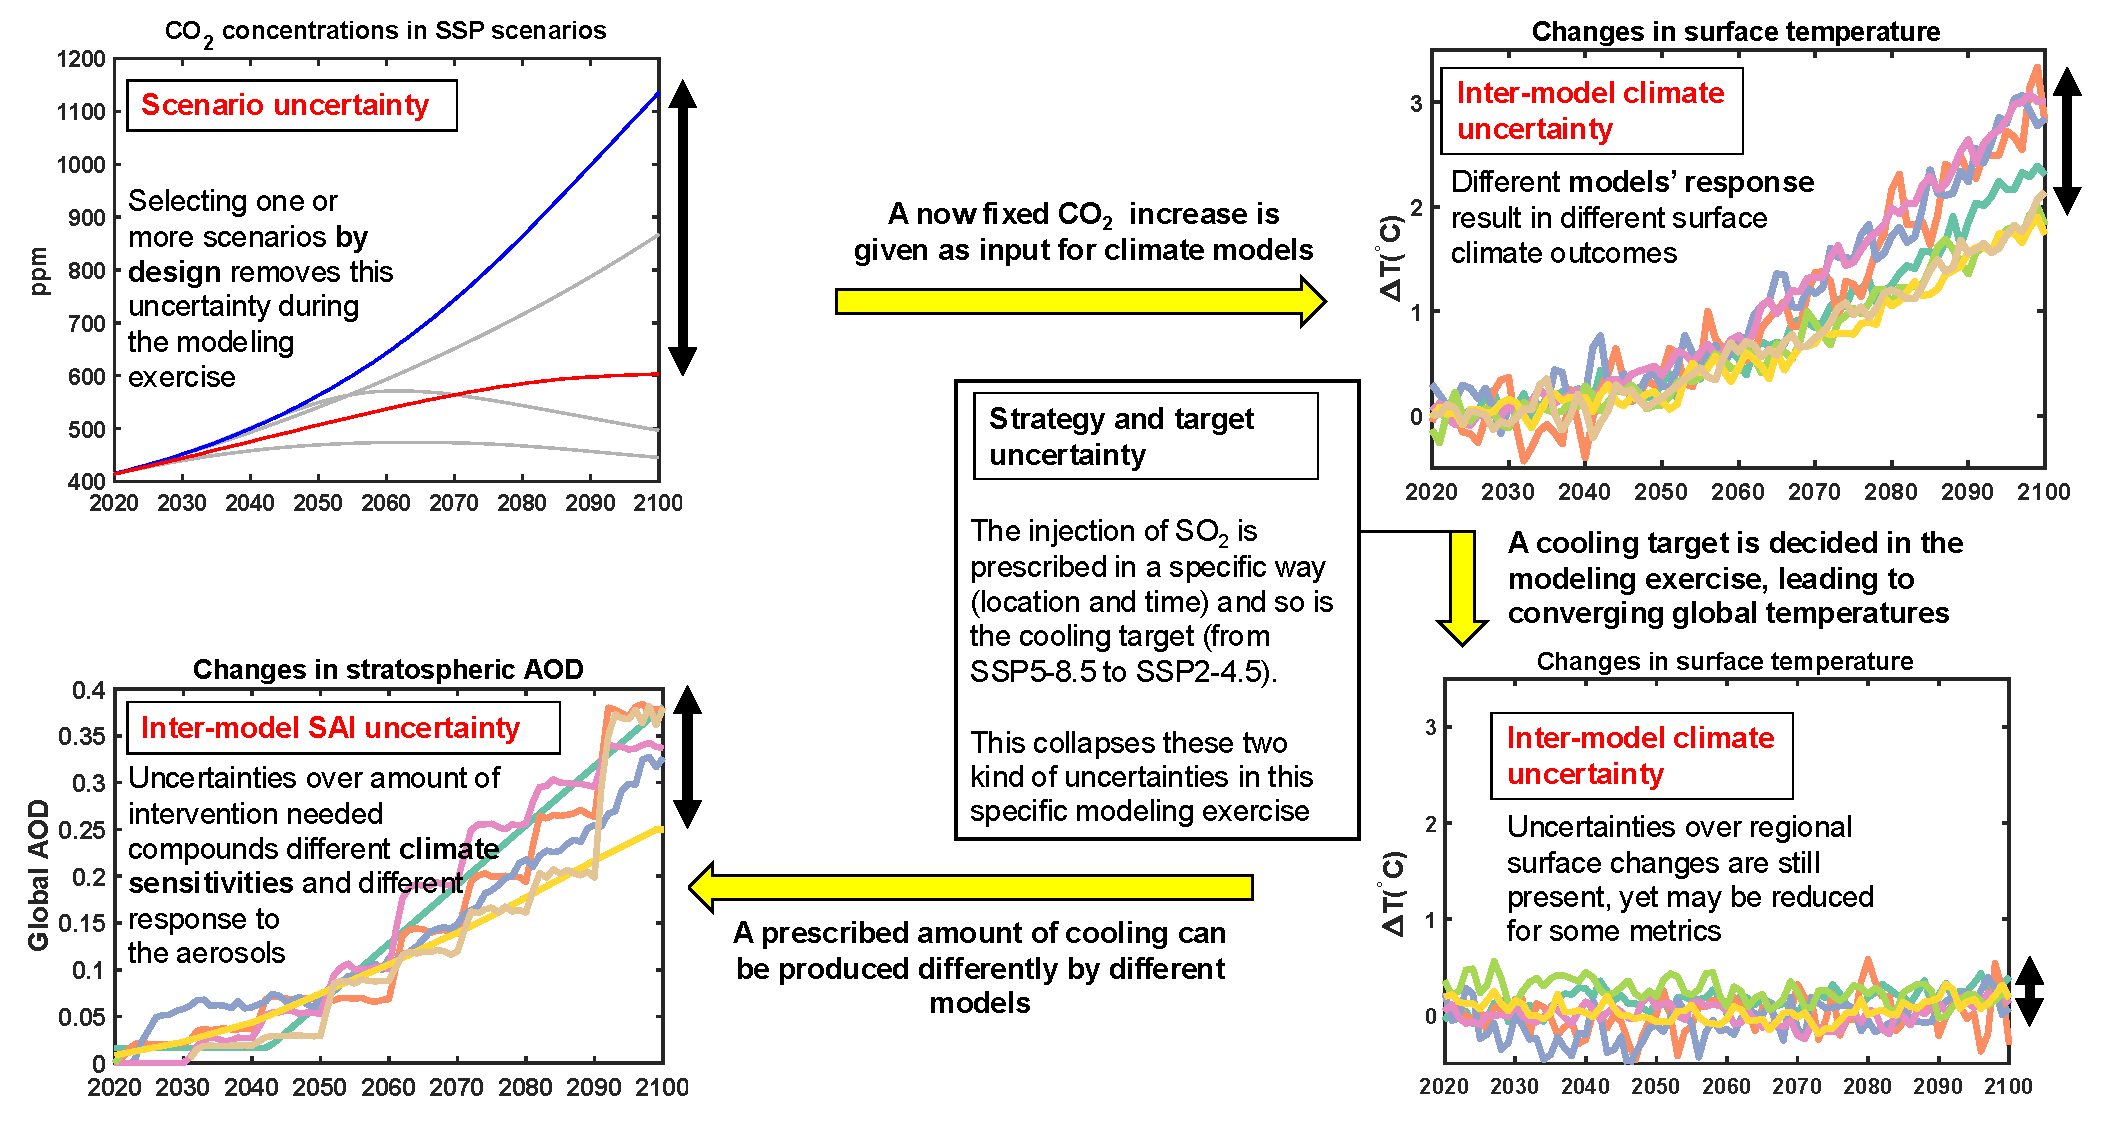
\includegraphics[width=14cm]{uncertainties_3.pdf}
\caption{Schematic figure explaining the ``collapsing'' or shifting of scenario uncertainty and of global scale inter-model uncertainty under multi-model SRM simulations.}\label{geomip_scheme}
\end{figure*}

\subsection{Inter-model SRM uncertainty: isolating aerosol uncertainties}

Isolating a specific inter-model SRM uncertainty can be challenging. In Earth System Model simulations, when multiple things are changing at once (GHGs, land use, tropospheric aerosols, as well as SRM deployment), disentangling a single cause of change without multiple sensitivity experiments can be difficult. At the same time, while simpler simulations in fixed-SST and/or time-slice setups can lead to the identification of specific sources of inter-model spread, they might fail to capture the whole range of interactions.

Here, we consider how inter-model SRM uncertainties can be better separated in the case of SAI. Using the G6solar and G6sulfur simulations we show how one can disentangle the uncertainties that specifically arise from differences in stratospheric aerosol responses. The solar dimming simulations (G6solar) can be considered as ``simpler'', in that the models all apply the forcing in the same way - a reduction in the solar constant implies the same geographical distribution of the top-of-atmosphere reduced forcing, even if their radiative code might threat the changes in radiation differently. In the SAI simulations (G6sulfur), on the other hand, even given the same level of global forcing, the aerosols are transported differently, and will have different sizes, meaning different scattering properties and lifetimes, leading to different geographical distributions of the top-of-atmosphere forcing, stratospheric perturbations and efficacy \citep{Tilmes2022}.

If one can envision an idealized case in which aerosol uncertainty is completely resolved, that is, one could apply the same aerosol distribution and the same radiative forcing to a specific aerosol distribution, the remaining inter-model uncertainty would be similar (to first order) to that of a solar dimming experiment. This excludes that, even given the same dynamical response in the stratosphere, there might be secondary responses to it that might differ (i.e. the same stratospheric heating might lead to different responses in the tropospheric circulation). However, we assume that such differences are small compared to the aerosol forcing itself, and that it is also compensated by the fact that, under solar dimming, the models would also be slightly different in their stratospheric responses \citep{Bednarz2022}. Nevertheless, the purpose here is not to perfectly identify and quantify all uncertainties, but to ascertain some form of separability so that we can identify which uncertainties are most important and how to resolve them.

\begin{figure*}[ht]
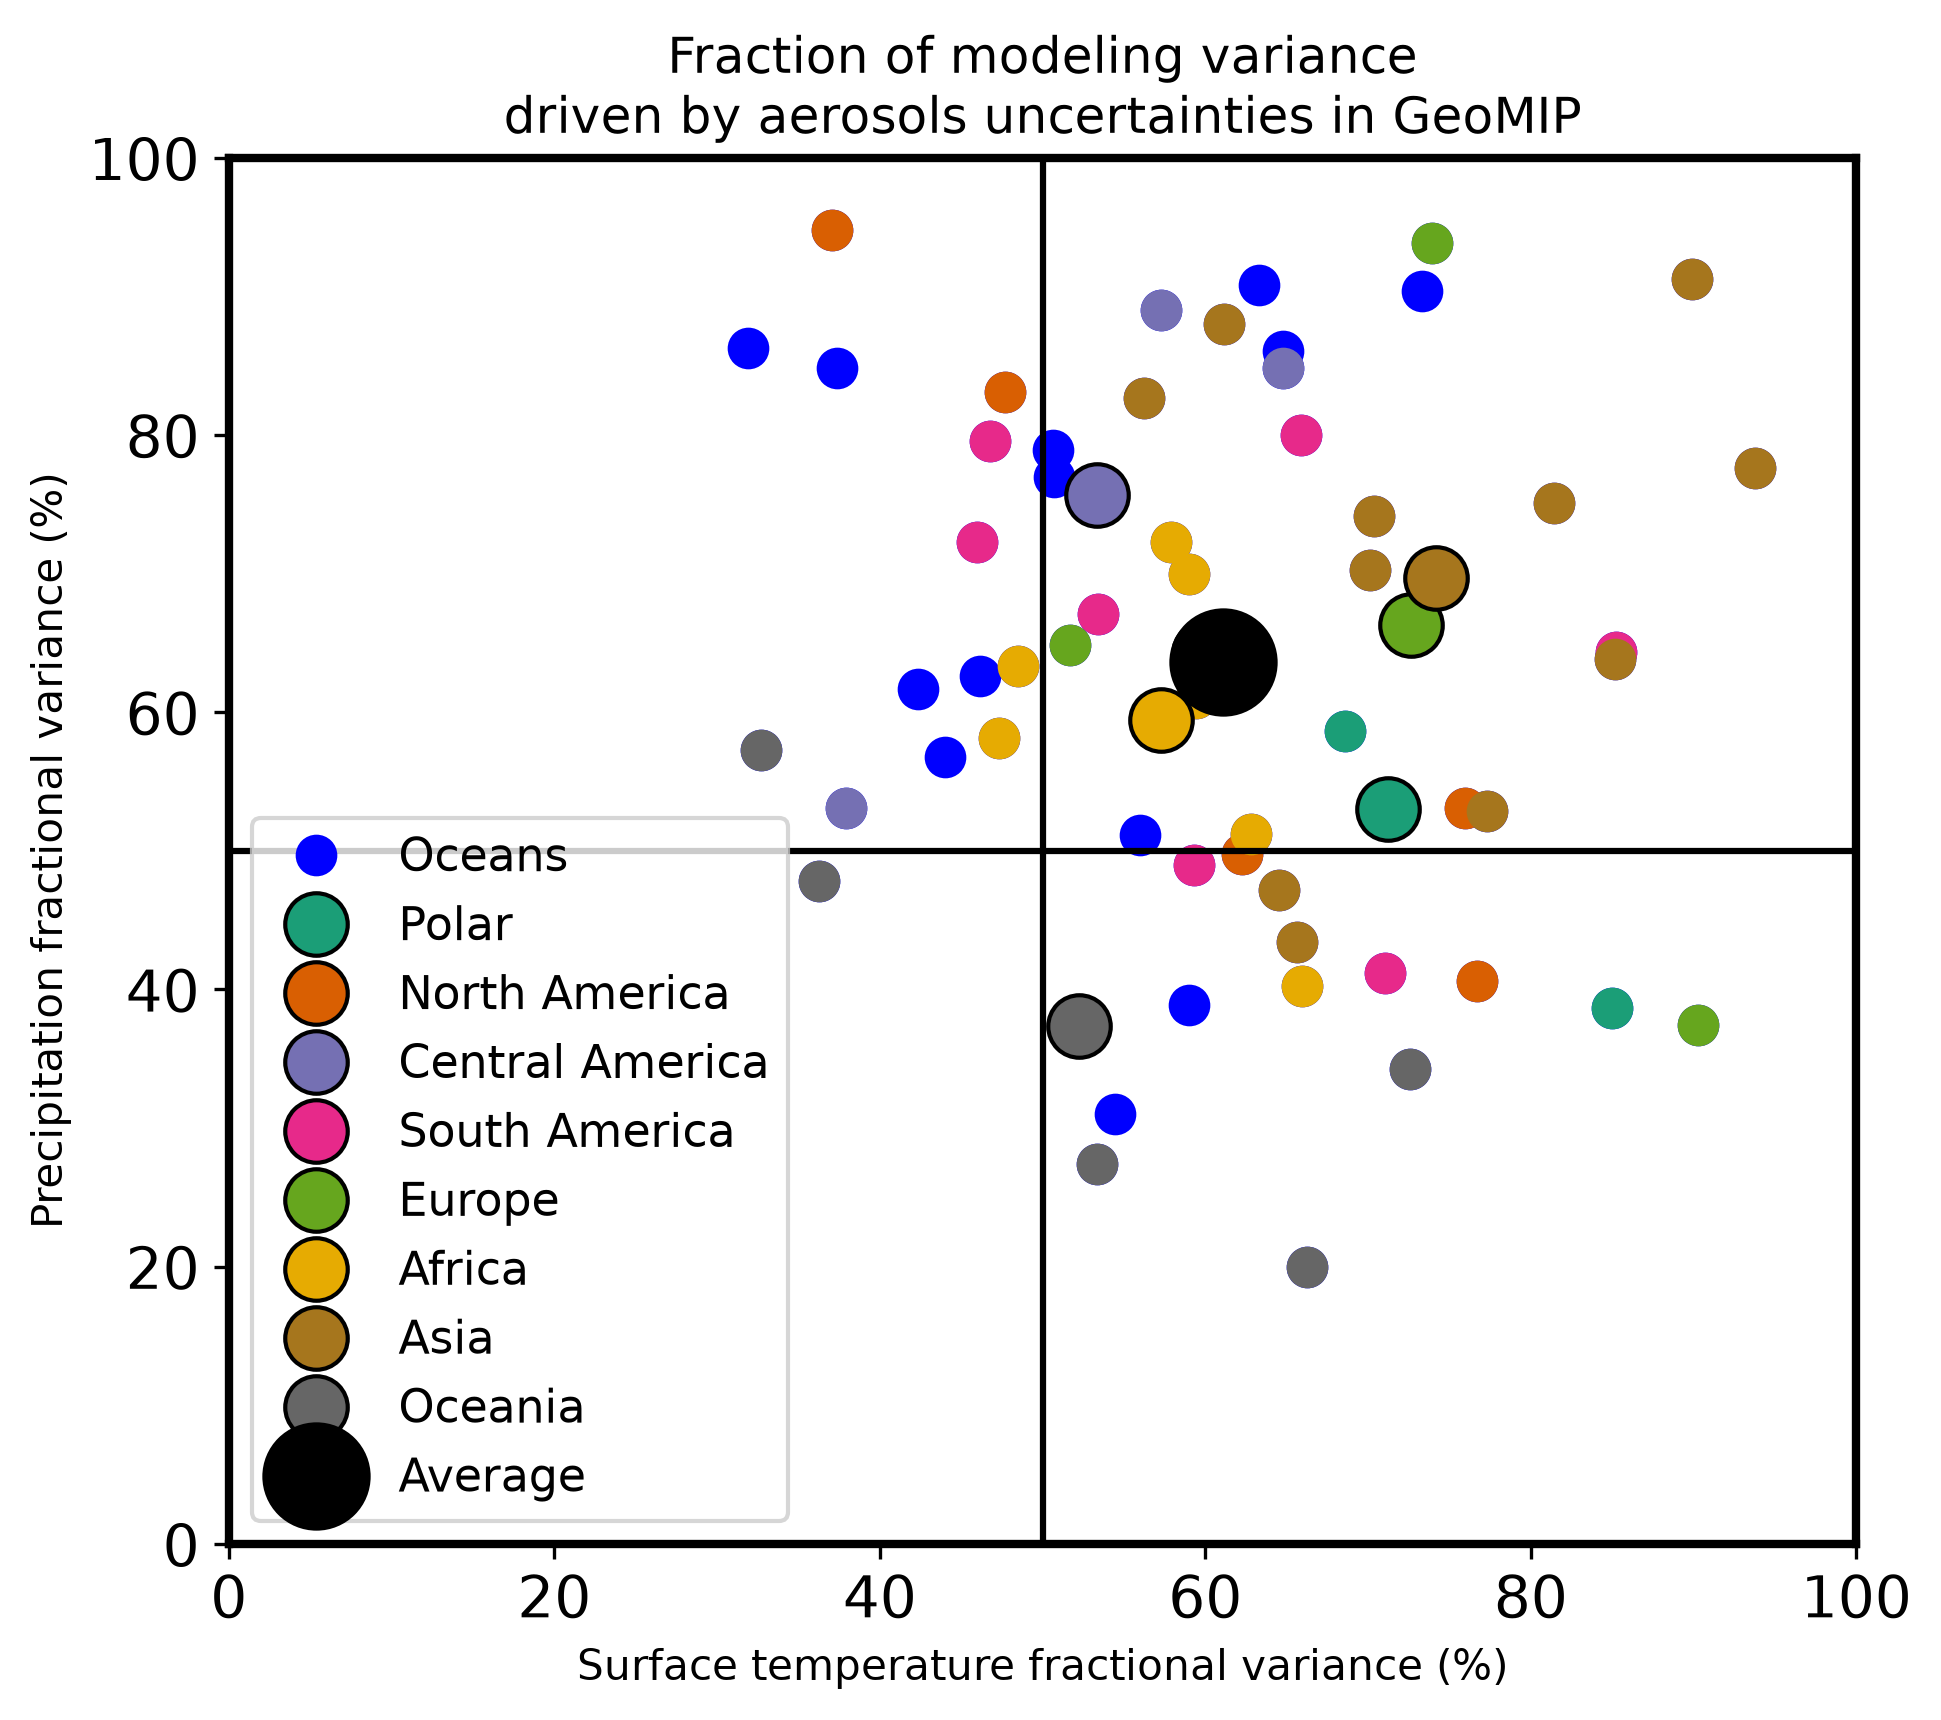
\includegraphics[width=0.8\linewidth]{figures/GeoMIP_uncertainties_aerosols.png}
\caption{Quantification of the fraction of model uncertainties driven by aerosol uncertainties in GeoMIP6 simulations, calculated as in Equation~\ref{eqn.frsulf}, using G6sulfur and G6solar inter-model spread results for the 2080-2100 period, and averaged over IPCC regions, here color-coded by continent for surface air temperature (tas) and mean precipitation (pr). The global value-aggregated from the regions is shown in black (61\% for surface air temperatures and 64\% for precipitation).}
\label{aerosols}
\end{figure*}

Using this approach, Fig.~\ref{aerosols} quantifies how much larger uncertainties are for SAI compared to solar dimming simulations. This is evaluated assuming that, if there was no added uncertainty due to the aerosols, the variance of the two different ensembles would be similar ($\sigma^2_{\mathrm{solar}} = \sigma^2_{\mathrm{sulfur}}$), and that the driver of the solar dimming uncertainty is the inter-model differences in the underlying climate responses due to the combination of climate change and SRM. If there is increased variance due to the aerosol uncertainties, then on average the fractional variance, calculated as
\begin{equation}\label{eqn.frsulf}
\mbox{fr}_{\mathrm{sulf}} = 1 -\frac{\sigma^2_{\mathrm{solar}}}{\sigma^2_{\mathrm{solar}}+\sigma^2_{\mathrm{sulfur}}}
\end{equation}
will be larger than 50\%. We find that in the vast majority of IPCC regions (75\%), uncertainties are higher when considering the simulations using aerosol injections for both surface temperature and precipitation, with only a few regions showing smaller values for one of the two variables, but none for the two combined: this means that the aerosol uncertainty drives a substantial part of the uncertainty, with global values of variance being on average 57\% higher for surface temperatures and 75\% higher for precipitation. 

\subsection{Inter-model uncertainties: Isolating differences in climatic feedbacks between warming and preventing warming}

While Fig.~\ref{aerosols} highlights the important driver of aerosol uncertainty in multi-model SRM simulations, it does not directly address how uncertainties from SRM compare to uncertainties under climate change. To do so, in this section we compare the G6sulfur increases in variance with the SSP5-8.5 ones. In \cite{Visioni2021}, it was already pointed out that inter-model spread for G6sulfur appeared to be smaller than inter-model spread for SSP5-8.5, mainly for surface temperatures and less so for precipitation \citep[e.g.,][]{MarMartin2015}. Here, we quantify this in a more robust way using a similar method as done in the previous section, by defining a potential increase in uncertainty through a quantification of increases in variance by comparing the two cases against the variance in the G6solar case:
\begin{align}
    &\mbox{Increase}_{\mathrm{sulf}} = \frac{\sigma^2_{\mathrm{sulfur}}}{\sigma^2_{\mathrm{solar}}}\label{eqn.increase.sulf} \\ &\mbox{Increase}_{\mathrm{ssp}} = \frac{\sigma^2_{\mathrm{ssp}}}{\sigma^2_{\mathrm{solar}}}\label{eqn.increase.solar}
\end{align}
calculated over the last 20 years of simulation (2080-2100). This compares the simulations G6solar (which is still not really in steady state), for which the amount of uncertainty is just due to different response in models to the compensation of longwave forcing from GHGs through a reduction in SW forcing, with G6sulfur, the compensation is spatially different due to the different aerosol distributions, leading to different climatic responses. Furthermore, we expand our analyses considering if different levels of spatial aggregation (here, exemplified by regridding the different model results to different horizontal resolutions) affect our conclusions. Analyzing different models, with their own specific resolution, always requires a regridding from a common grid, and this provides us with an opportunity to test if our analyses of uncertainty are affected. This is particularly important as, in other cases, we aggregate the results we show by either continent or IPCC region for ease of display.

In Fig.~\ref{aggregation}, which plots Equations~\ref{eqn.increase.sulf}-\ref{eqn.increase.solar}, we find some important results. Firstly, for both  surface temperature and precipitation, overall uncertainty is lower for the SAI simulations compared to the one with increased warming. In particular, with higher levels of uncompensated warming, uncertainties in local temperature changes are (compared with the median value of the solar reduction case) 120\% higher, whereas for SAI the uncertainties are 55\% higher. For precipitation, our analyses show that there is still a large uncertainty even under the G6solar case, and the increase in uncertainty driven by the uncompensated warming is 50\% higher, whereas it is 25\% higher for the compensated case with SAI. Summarizing, SAI-driven uncertainties in GeoMIP modeling results are roughly half as large as GHG-driven uncertainties. The median value we obtain (which is more appropriate here to use given the large number of points, hence being less sensitive to outliers, which can also be affected by internal variability) is, importantly, not sensitive to different degrees of spatial aggregation: whether considering a common 15$^{\circ}$ grid, the changes in variance are the same as when considering a 1$^{\circ}$ grid. Nevertheless, when considering smaller regions (such as a 1$^{\circ}$ pixel), the single results will be greatly affected by internal variability, so our results do not imply that uncertainty does not grow larger with smaller regions: rather, that as a whole, differences in uncertainties between the cases are not sensitive to the spatial aggregation chosen. While our choice of aggregation is not the same as a statistical or dynamical approach to downscaling, it can provide some insight to what one could expect when such methods are applied to coarse-resolution SRM modeling results: that the overall partitioning of uncertainty between downscaled simulations of SRM compared to downscaled simulations of climate change should not be qualitatively different (i.e. that the ratio in the spread of potential outcomes between the two should remain similar). While there is a paucity of such downscaling efforts for now, initial results seem to suggest this is true \citep{Sun2026}.

\begin{figure*}[ht]
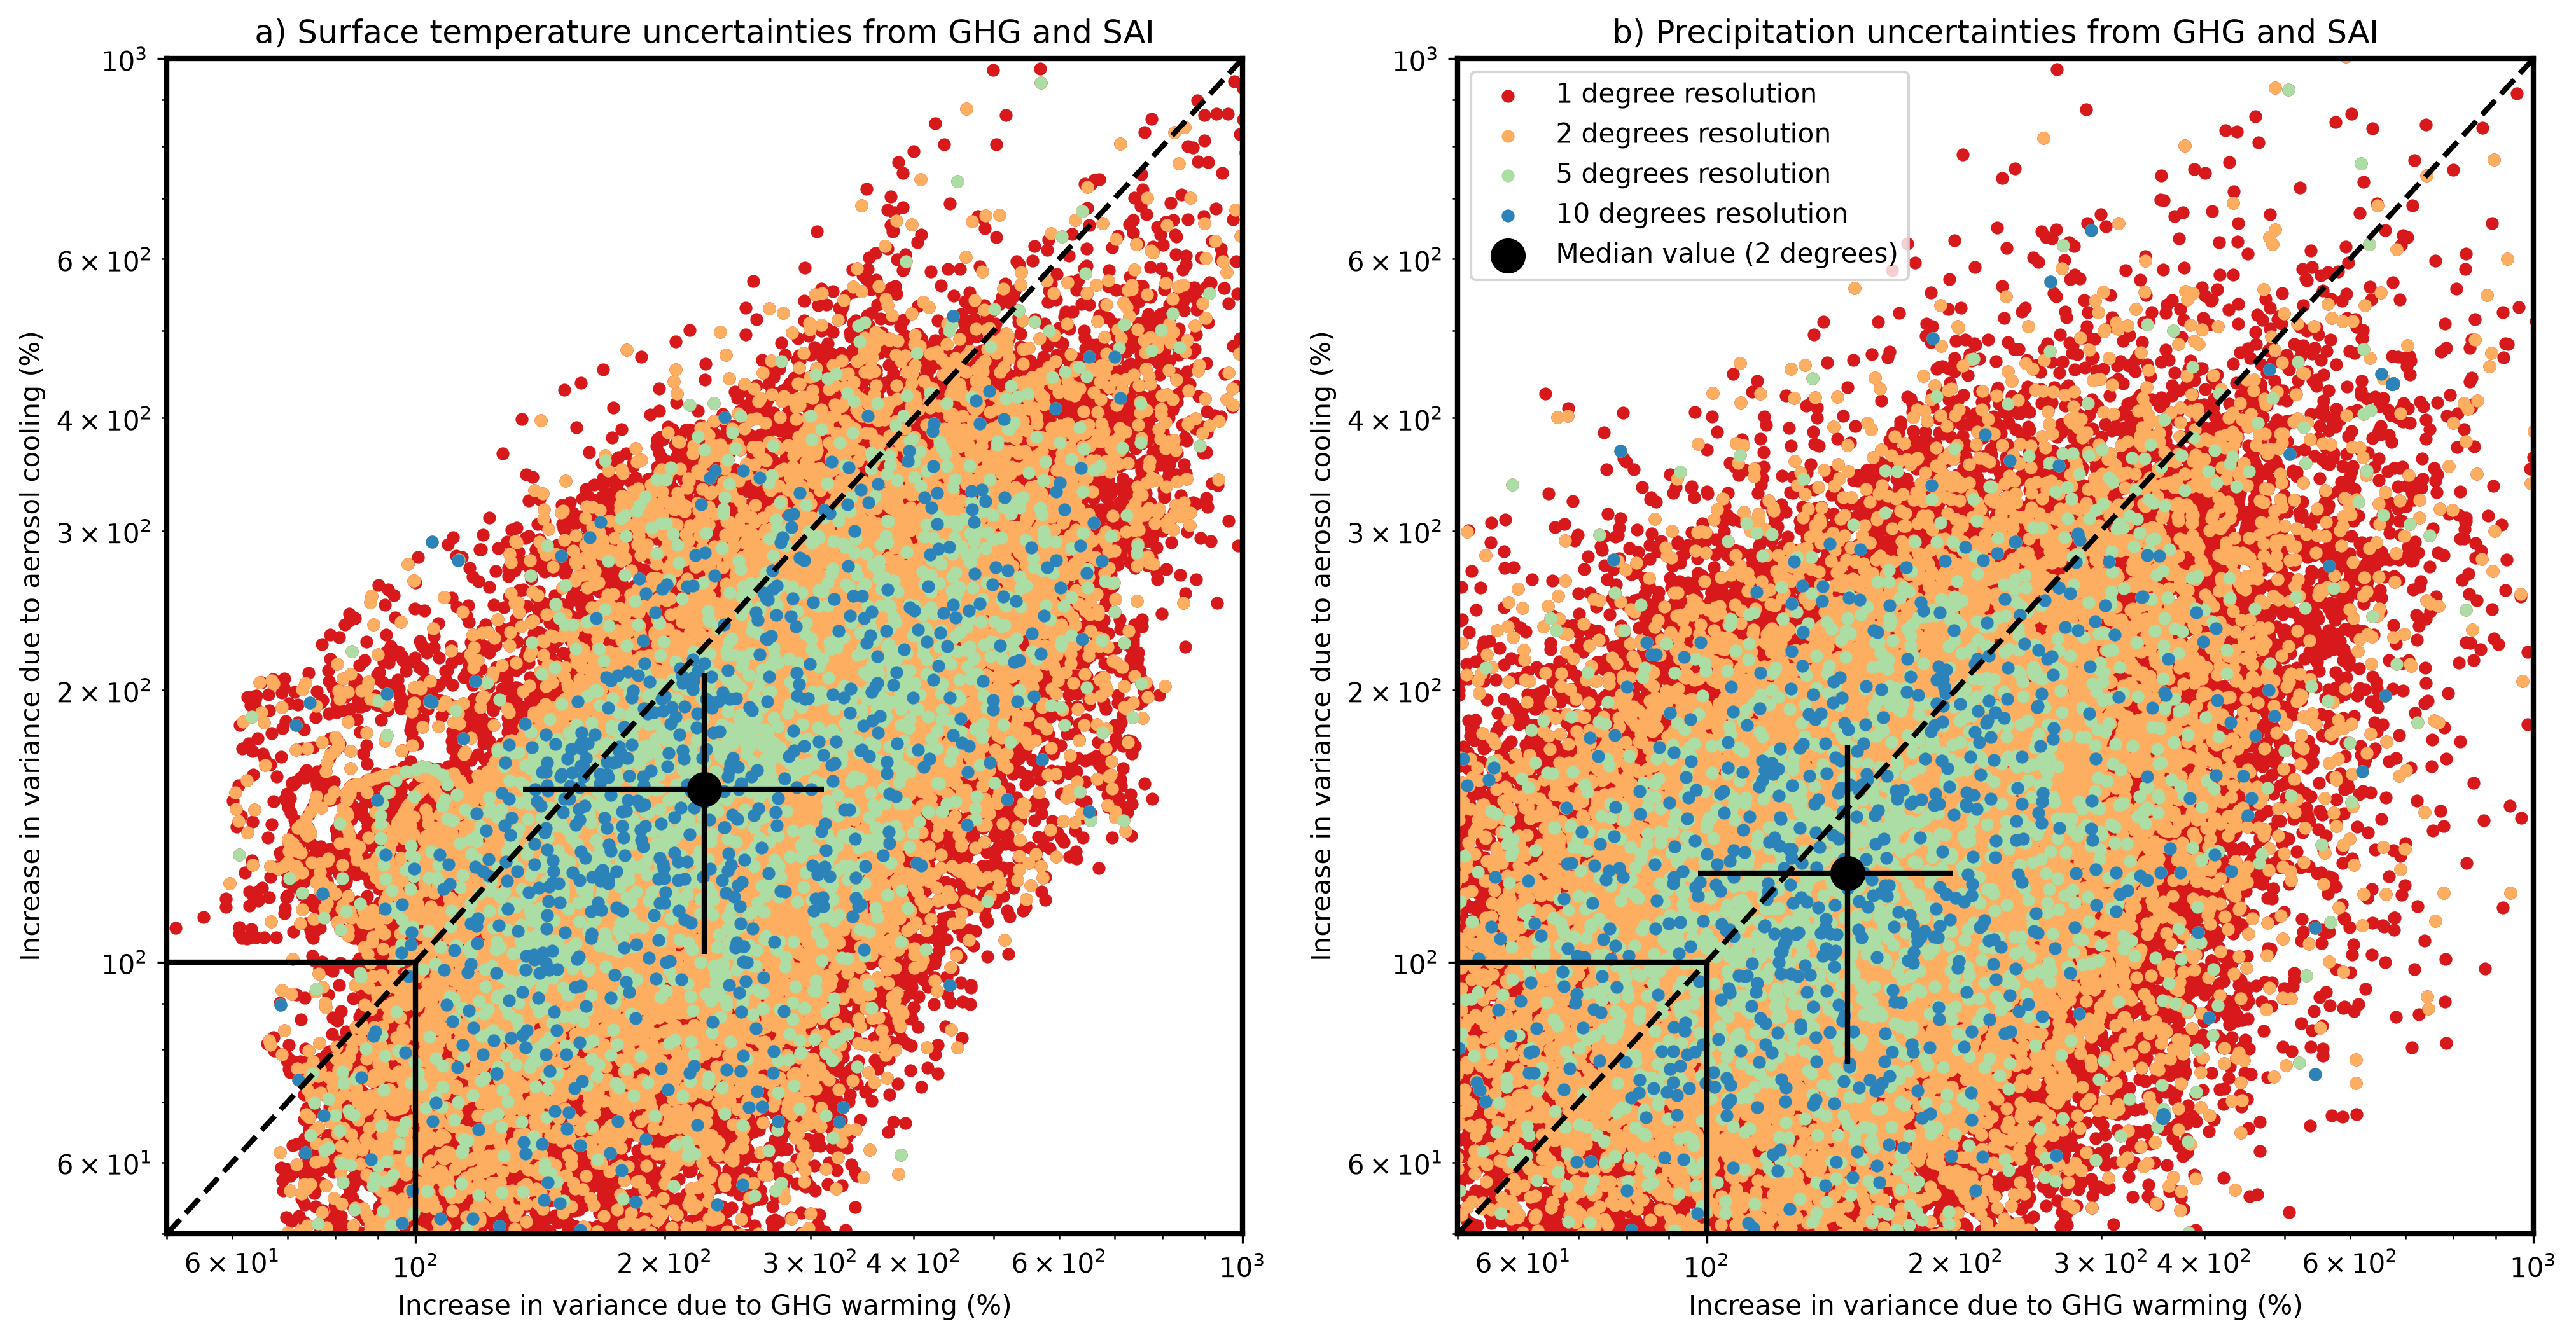
\includegraphics[width=14cm]{figures/GeoMIP_spatial_uncertainties.png}
\caption{Scatter plots of inter-model variance (calculated from Equations~\ref{eqn.increase.sulf}-\ref{eqn.increase.solar}) under higher warming and under SAI per each grid-box (with different colors indicating different spatial aggregation, see legend), for surface air temperature (panel a) and precipitation (panel b) considering the 2080-2099 period. The black point represent the median value for the cloud of points for the 1 degree resolution, with error bars represent the 98 percentile of the distribution.}
\label{aggregation}
\end{figure*}

\subsection{Uncertainties in the climatic response to different aerosol types}

We now define our overall uncertainty as $\sigma^2_{\mathrm{tot}} = 
\sigma^2_{\mathrm{solar}}+\sigma^2_{\mathrm{sulfur}}+\sigma^2_{\mathrm{aerosols}}$ to identify how much the inclusion of other aerosols affects the overall uncertainty. To compute this, we use $\sigma^2_{\mathrm{solar}}$ and $\sigma^2_{\mathrm{sulfur}}$ as before from the G6sulfur ensemble and calculate $\sigma^2_{\mathrm{aerosols}}$ as the variance in results across different aerosol types from the SOCOL ensemble.

We provide an example of our analyses for the IPCC African regions in Fig.~\ref{africa_socol}, including for informational purposes also SSP5-8.5 variance across the GeoMIP ensemble. Africa is the only region, as already pointed out in \cite{Visioni2021}, where variance was high even under G6solar, so it is an interesting case. For temperature, the difference in warming (from the baseline) ranges between 1 and 2 K, whereas G6solar and G6sulfur show similar, yet smaller, uncertainties, which are centered around 0 K by design, as the global target is correctly reflected in the regional multi-model mean. The SOCOL results present much smaller uncertainties for the aerosol material itself, which makes sense if we consider that temperature changes are more directly driven by where the aerosols are, rather than their type, which would mainly affect secondary impacts such as stratospheric heating-induced surface changes. For precipitation, the situation is more complex and highly heterogeneous. This indicates both the importance of more localized assessments, including a mechanistic understanding of the local drivers, as well as care in making broader assessments about continent-level impacts. 

\begin{figure*}[ht]
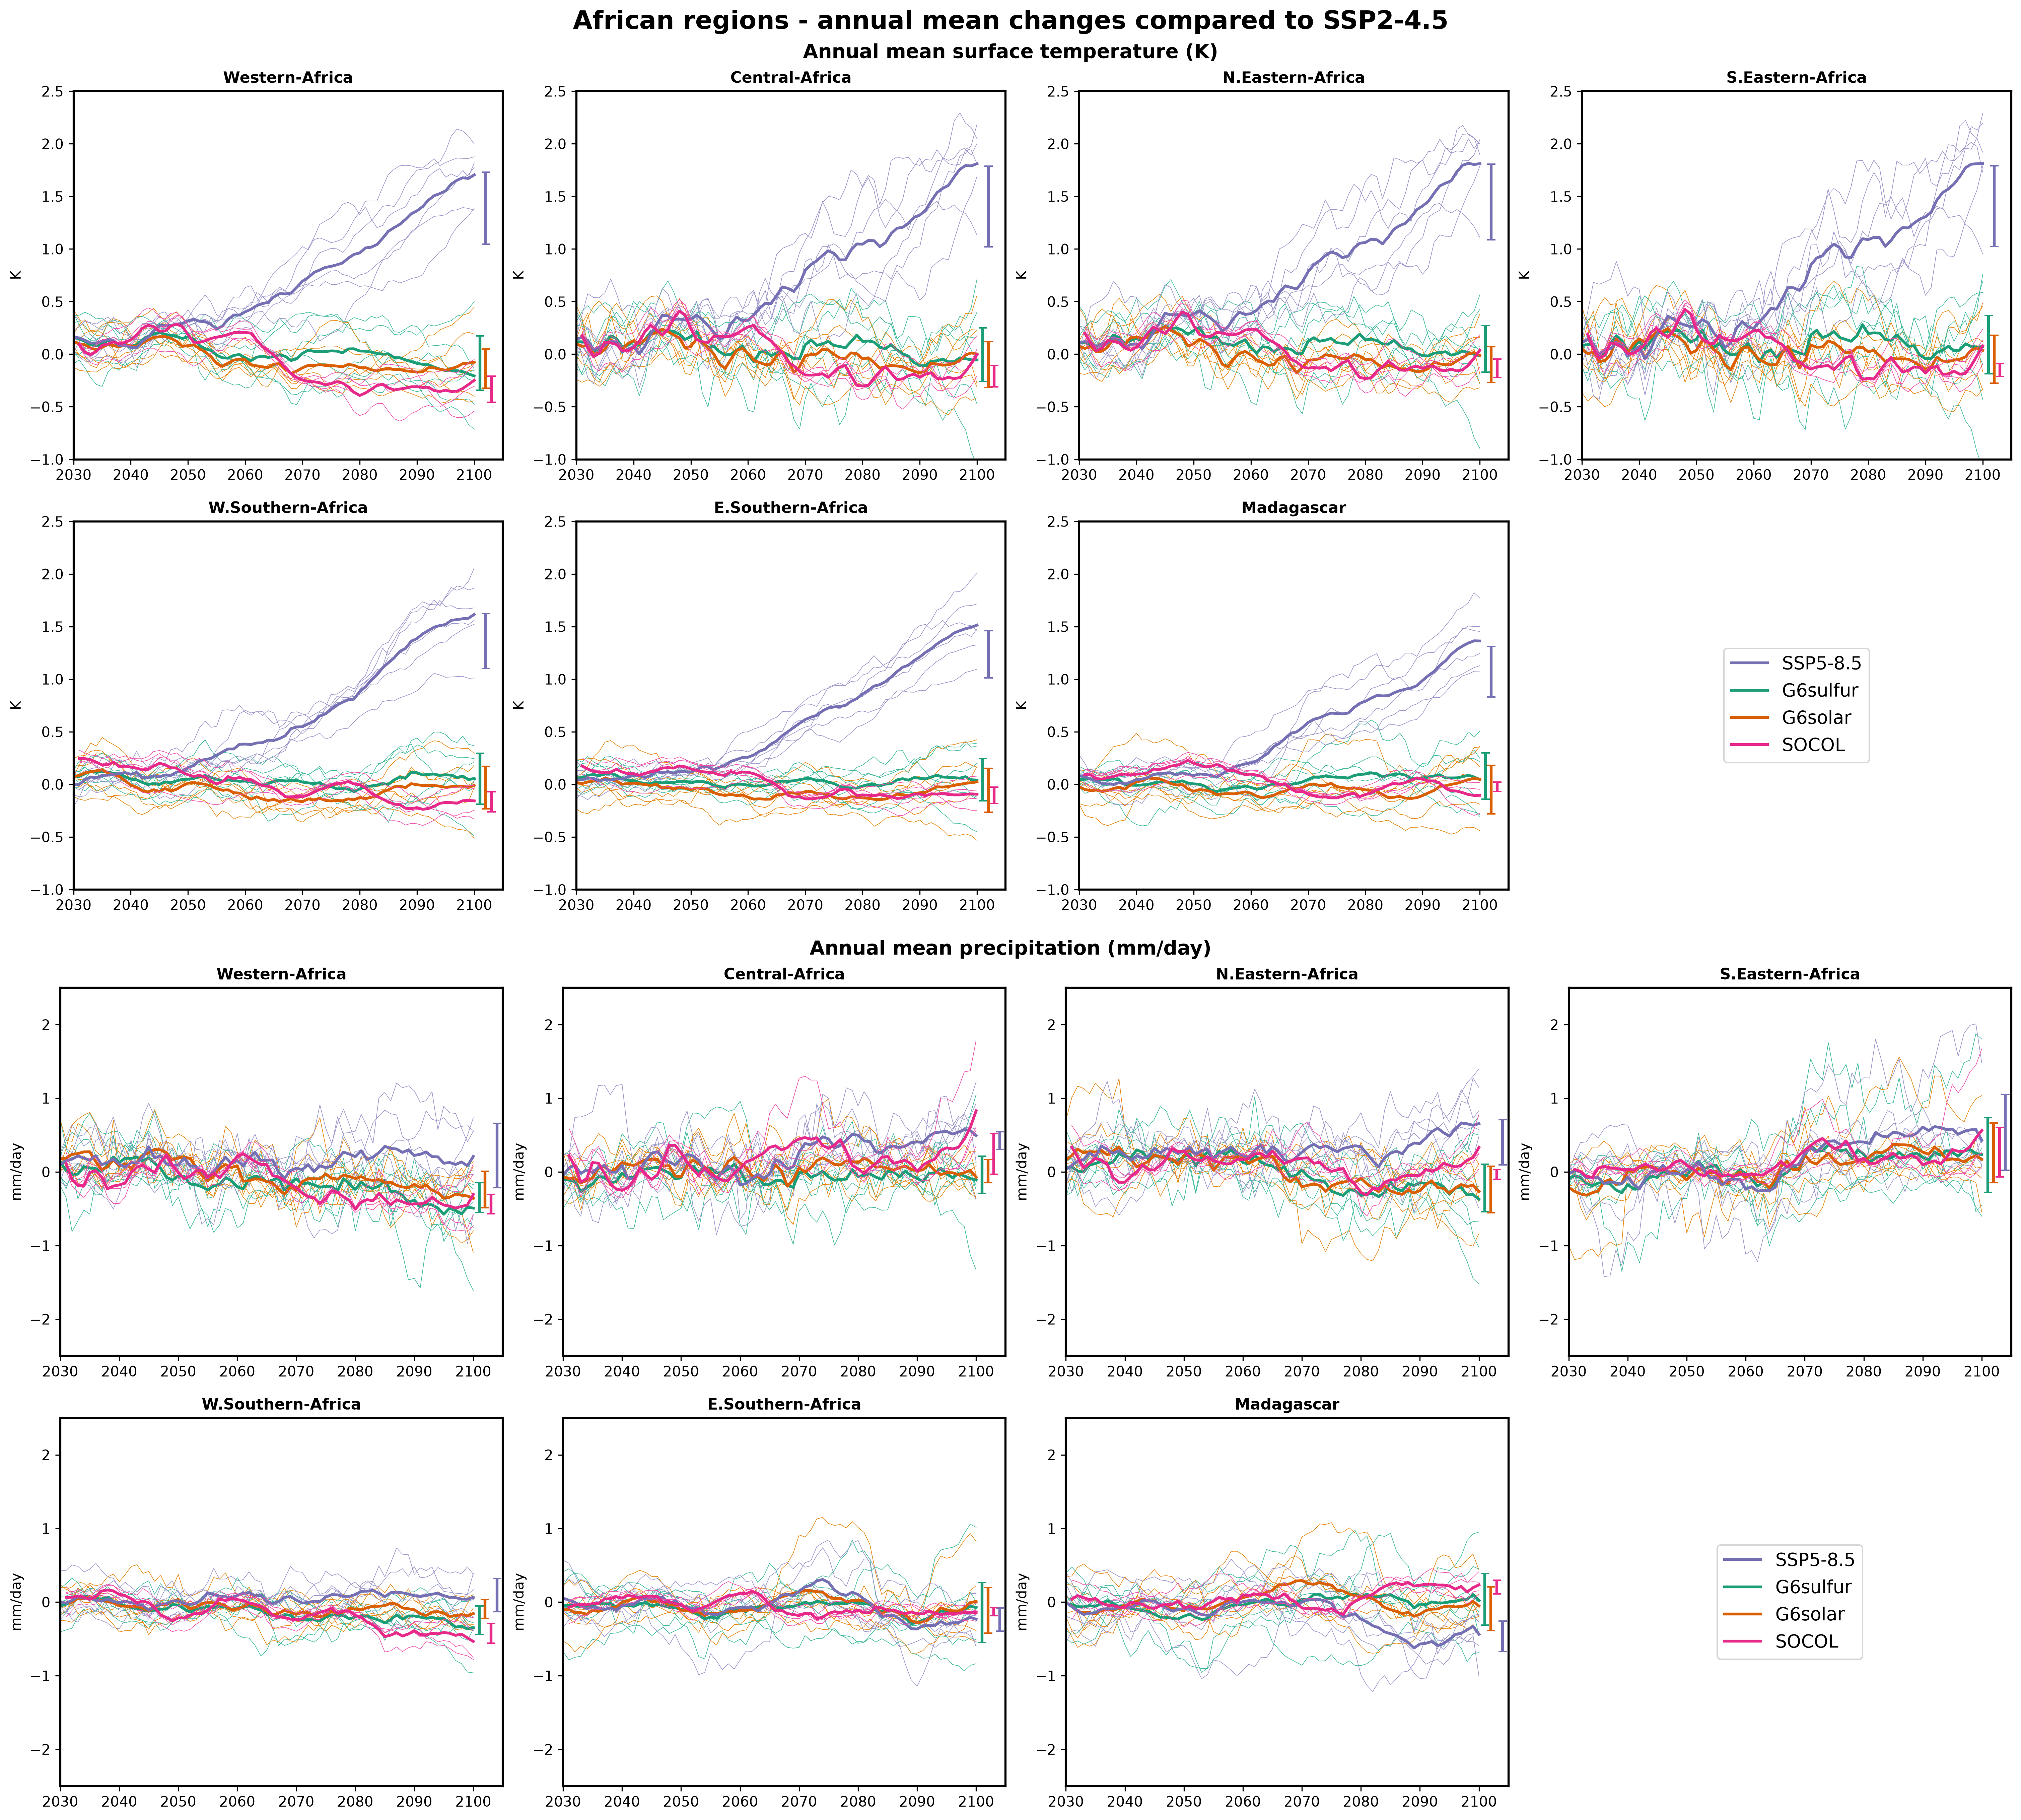
\includegraphics[width=0.95\linewidth]{figures/Africa_SOCOL.png}
\caption{Annual mean surface temperature changes (top panels) and annual mean precipitation changes (bottom panels) in the 7 Earth System Models in GeoMIP6 (including SOCOL) compared to SSP2-4.5 in each African IPCC region. Lighter lines represent ensemble means per each model, while thicker lines represent the multi-model ensemble. Standard deviation for the multi-model ensembles for the period 2080-2099 is shown on the right of each plot.}
\label{africa_socol}
\end{figure*}

The results for the partitioning of the overall uncertainty for all IPCC regions is shown in Fig.~\ref{socol_uncertainty}. Overall, this shows a broad consistency with results highlighted for Africa for temperature, with most of the uncertainty driven by overall aerosol uncertainties, whereas for precipitation, Europe presents a clear outlier, with a larger fraction of the uncertainty driven by the aerosol type rather than only by aerosol uncertainties, potentially driven by the sensitivity of European precipitation to the North Atlantic Oscillation (NAO), and the potential impacts of stratospheric heating on the NAO \citep{Jones2022,Banerjee2021}.

\begin{figure*}[ht]
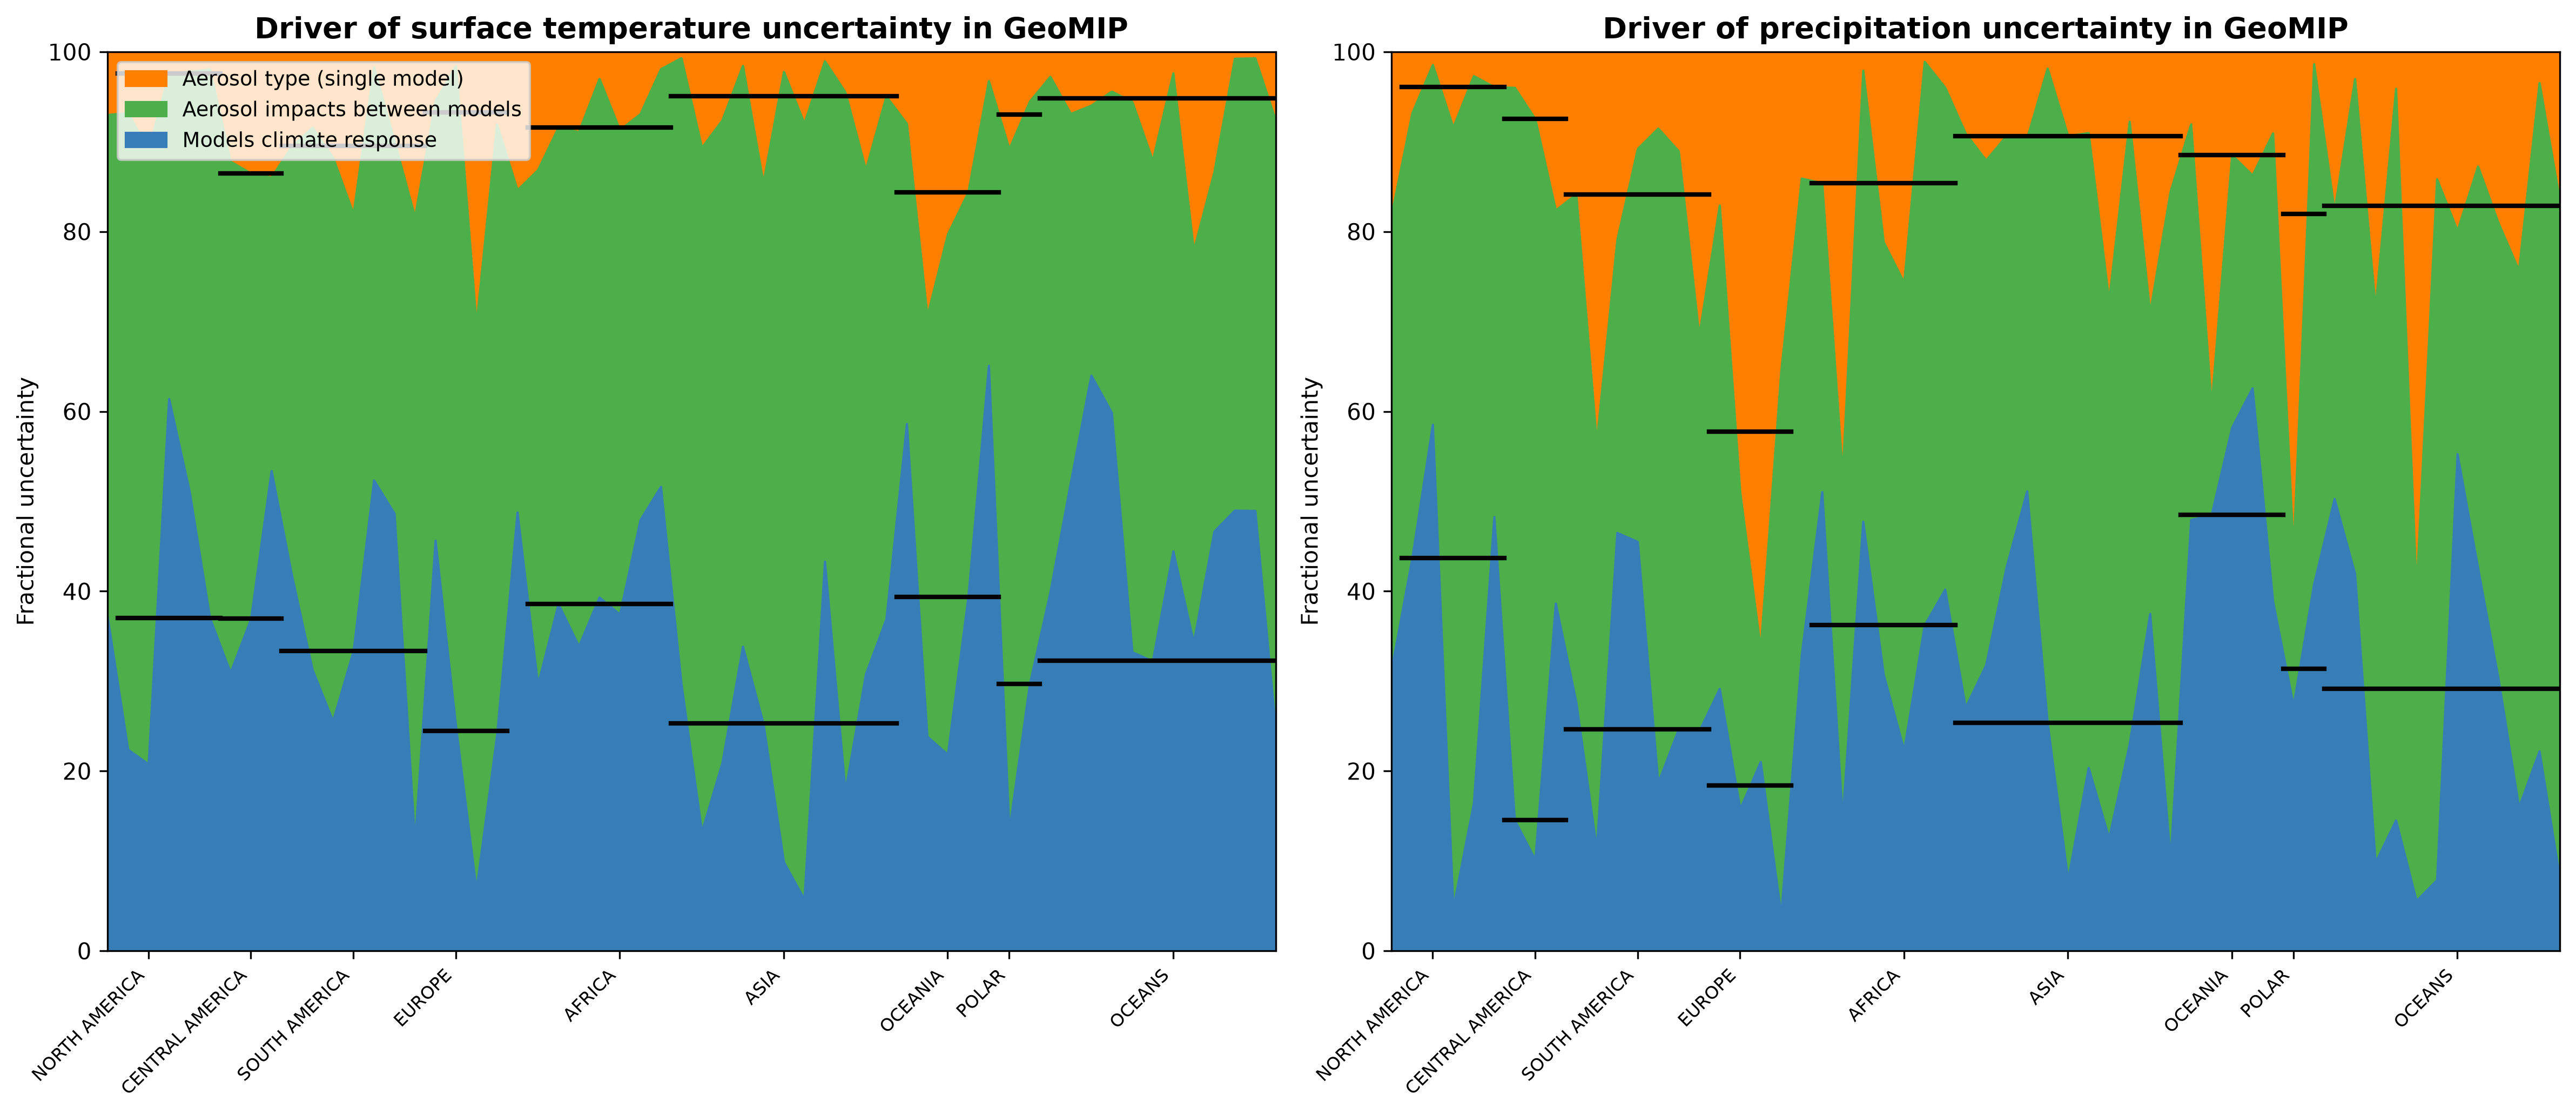
\includegraphics[width=0.95\linewidth]{figures/GeoMIP_uncertainties_aerosols_SOCOL_tas_pr.png}
\caption{Assessment of fractional variance (with $\sigma^2_{\mathrm{tot}} = \sigma^2_{\mathrm{solar}}+\sigma^2_{\mathrm{sulfur}}+\sigma^2_{\mathrm{aerosols}}$) for the GeoMIP6 ensembles, including SOCOL simulations with different aerosol types, for surface air temperature (panel a) and precipitation (panel b) for the 2080-2099 period. The x-axis in both plots shows each different IPCC region, whereas the continent-level average is shown with a thick black line (also labeled on the x-axis).}
\label{socol_uncertainty}
\end{figure*}

\clearpage

\subsection{Scenario, strategy and target uncertainty}

As remarked in the previous sections, the choice of a specific temperature target in SRM simulations collapses the uncertainty related to the global modeled temperature response to GHGs. What the G6 GeoMIP simulations can't do is help us understand what is the uncertainty of models' response to different targets and strategy, as they sub-select for one single scenario. In this section therefore we look at results for one single model (CESM2-WACCM) for which multiple strategies and targets are available. Building on work by \cite{zhang_how_2022}, Figs.~\ref{strategy_tas} (surface temperature) and \ref{strategy_pr} (precipitation) show how uncertainty across these other dimensions can inform total uncertainty, calculated as
\begin{equation}
\sigma^2_{\mathrm{tot}} = \sigma^2_{\mathrm{strategy}}+\sigma^2_{\mathrm{scenario}}+\sigma^2_{\mathrm{internal}}
\end{equation}
where $\sigma^2_{\mathrm{internal}}$ is calculated using the ensemble spread for all simulations, which include three ensemble members each. At the global level, we find for both temperature and precipitation that the decision of a specific target is the main driver of the uncertainty, with strategy and internal variability playing only a very small part (less than 10\% for temperature, 25 \% for precipitation).

\begin{figure*}[ht]
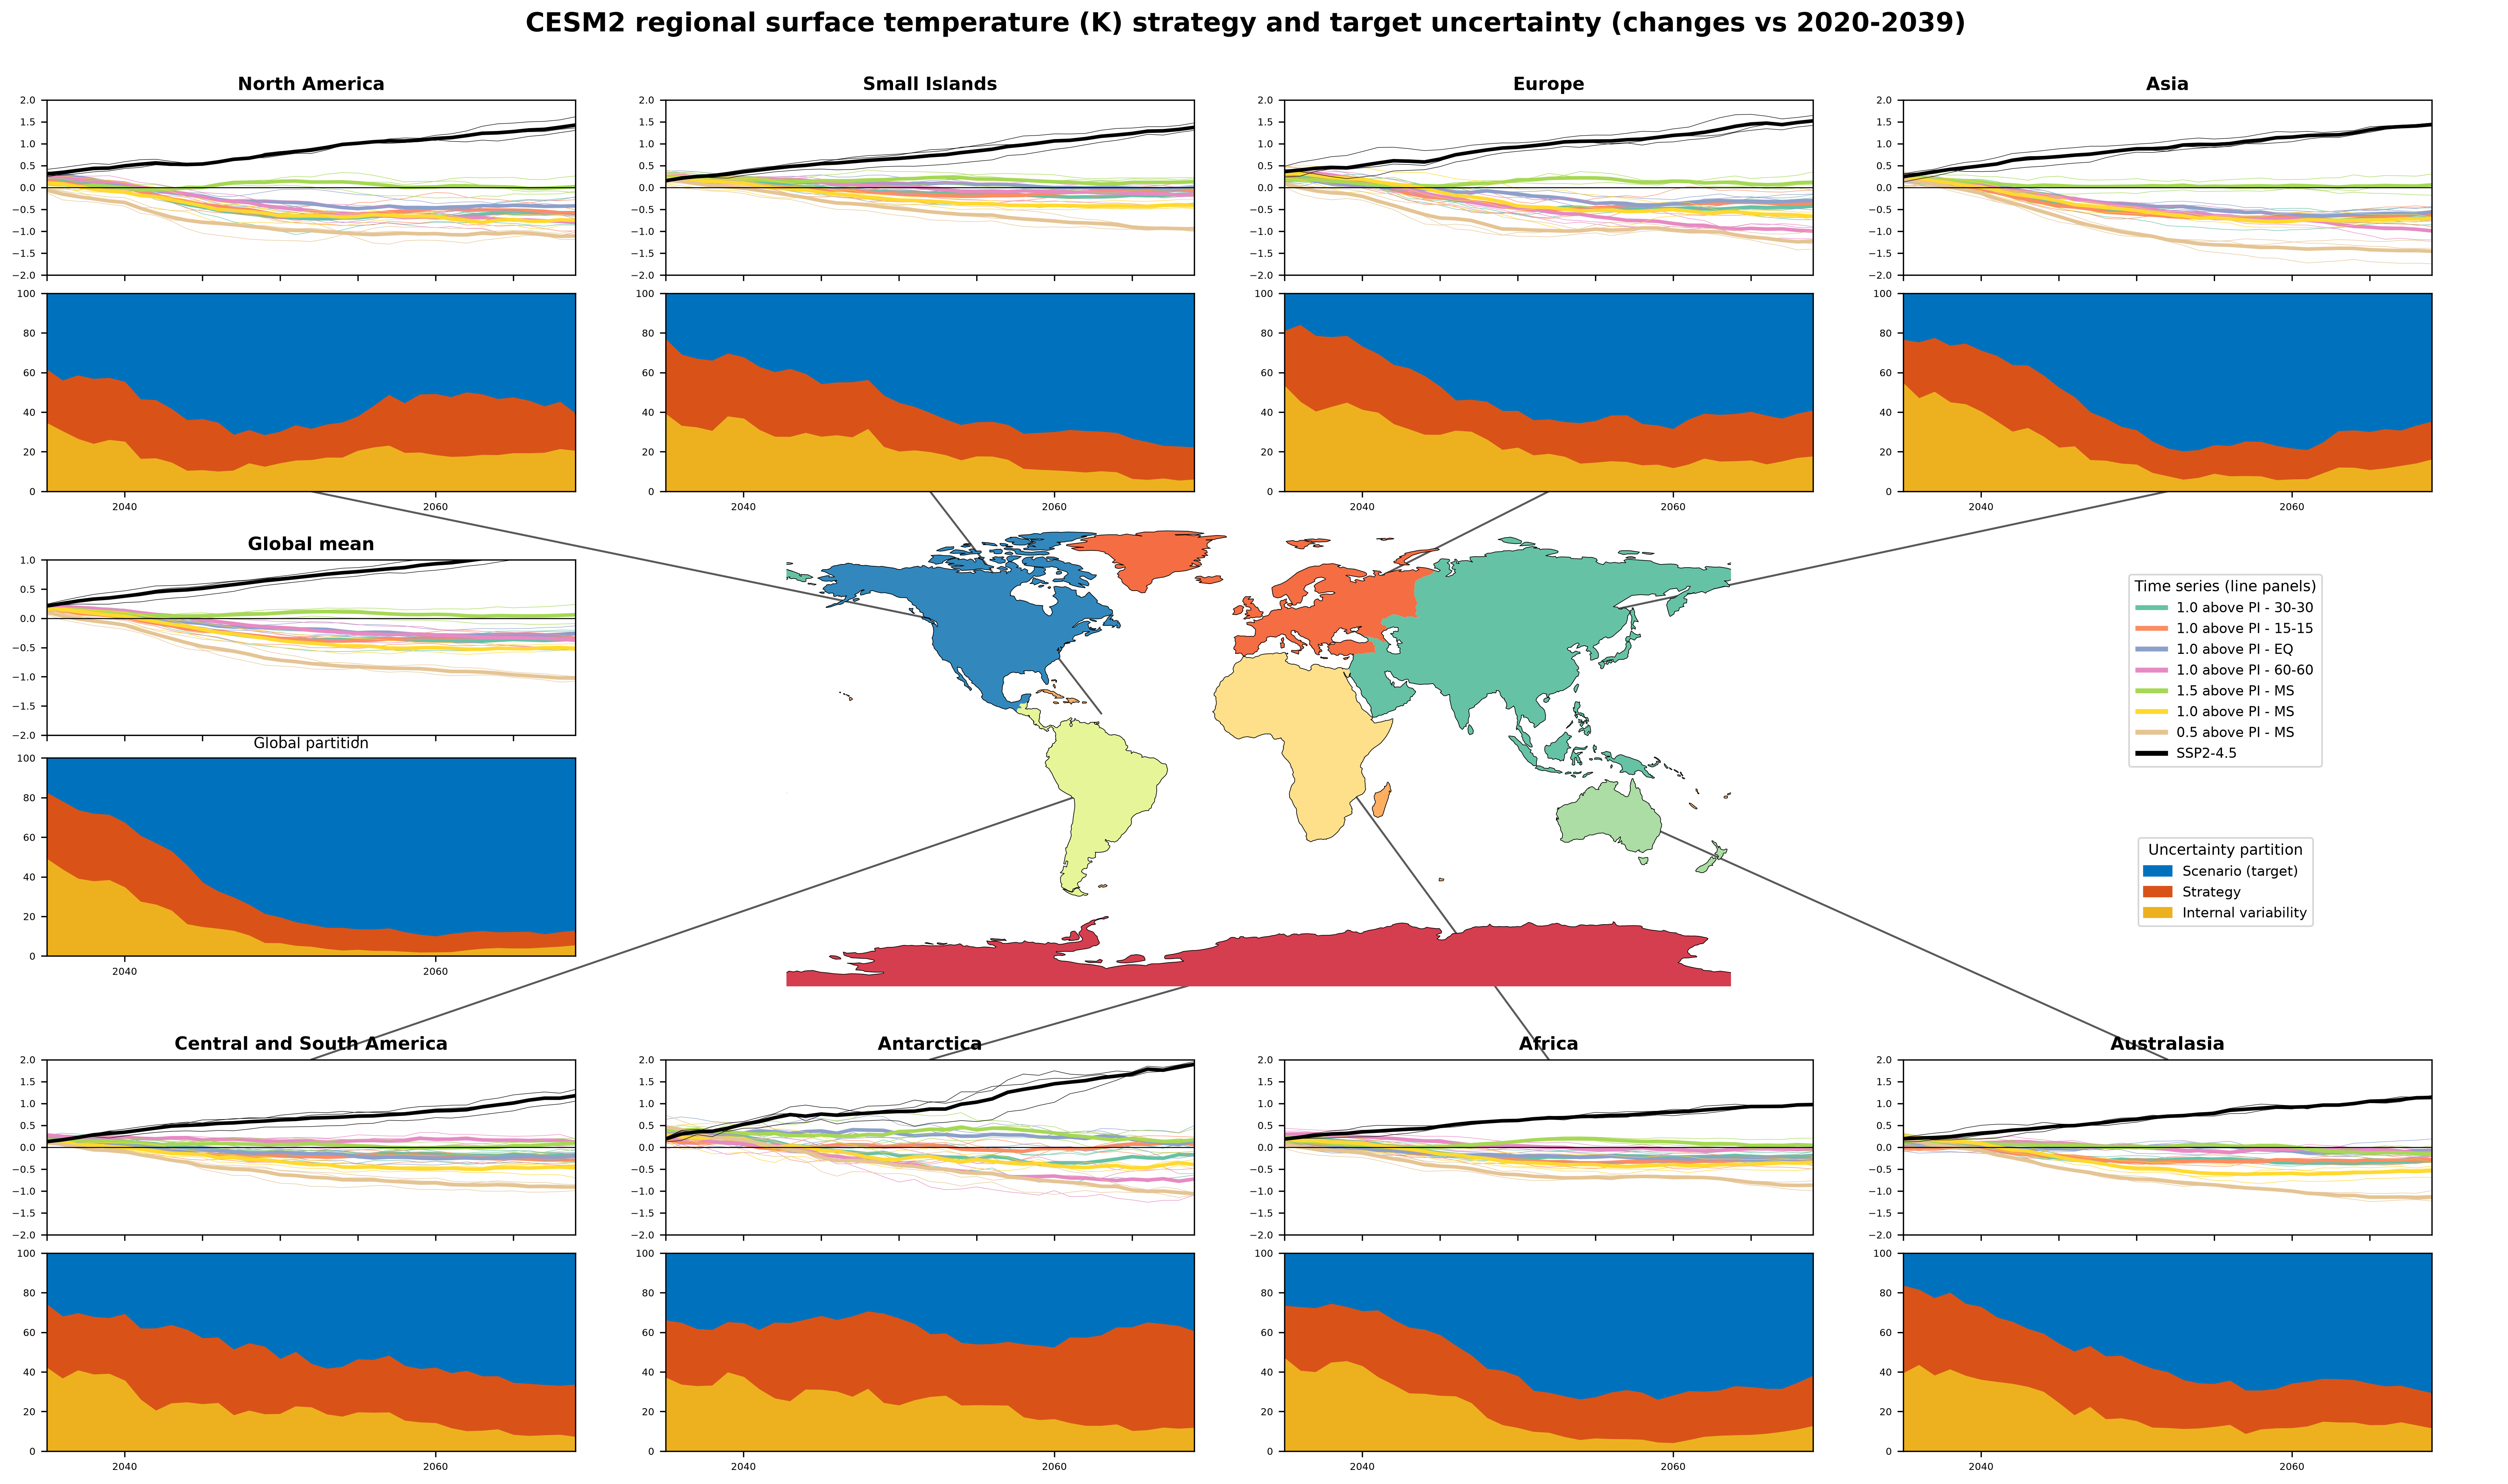
\includegraphics[width=0.95\linewidth]{figures/HS_plot_TREFHT_regions_map.png}
\caption{Partitioning of scenario, strategy, and internal uncertainties at the global (top left) and continental levels for annual mean surface air temperatures. For each region, values of the changes compared to the period 2010-2029 are shown (above), color-coded by strategy and scenario (see legend), whereas the bottom plot shows the partitioning given the values above.}
\label{strategy_tas}
\end{figure*}

At the continental level, our analyses show a very distinct behavior for temperature (Fig.~\ref{strategy_tas}) and precipitation (Fig.~\ref{strategy_pr}). For temperature, on every continent except Antarctica, the scenario uncertainty still plays the largest role (more than 50\% in all regions), with strategy uncertainty and internal variability contributing substantially, but differently by continent. For instance, over North America, strategy uncertainty contributes 23\% in the 2050-2069 period, and internal variability for 20\%, whereas in Asia and Europe the strategy uncertainty is smaller (around 17\%). The particular sensitivity of Antarctic temperature to strategy can be explained by the presence of a more ``polar'' strategy (injections at 60$^{\circ}$N and 60$^{\circ}$S) that act as a distinct way to cool higher latitudes. 

Moving to precipitation, we can see that different continents present much larger differences. In South and Central America, the regional precipitation changes are greatly driven by the target uncertainty (just as much as for temperature), whereas in North America and Africa the strategy uncertainty plays as much of a role as the target uncertainty. In all cases, internal variability at the continental level is at least 20\%. Importantly, our results suggest that such uncertainty is not always a function of the magnitude of deployment; that is to say, in most regions, the strategy uncertainty is as relevant in the first decade of deployment as after 30 years. This would have important consequences both imagining the potential preference of a continent for a specific strategy over another and for its implication on how to detect whether a specific chosen strategy is being effective at its intended precipitation target at a regional level. 

\begin{figure*}[ht]
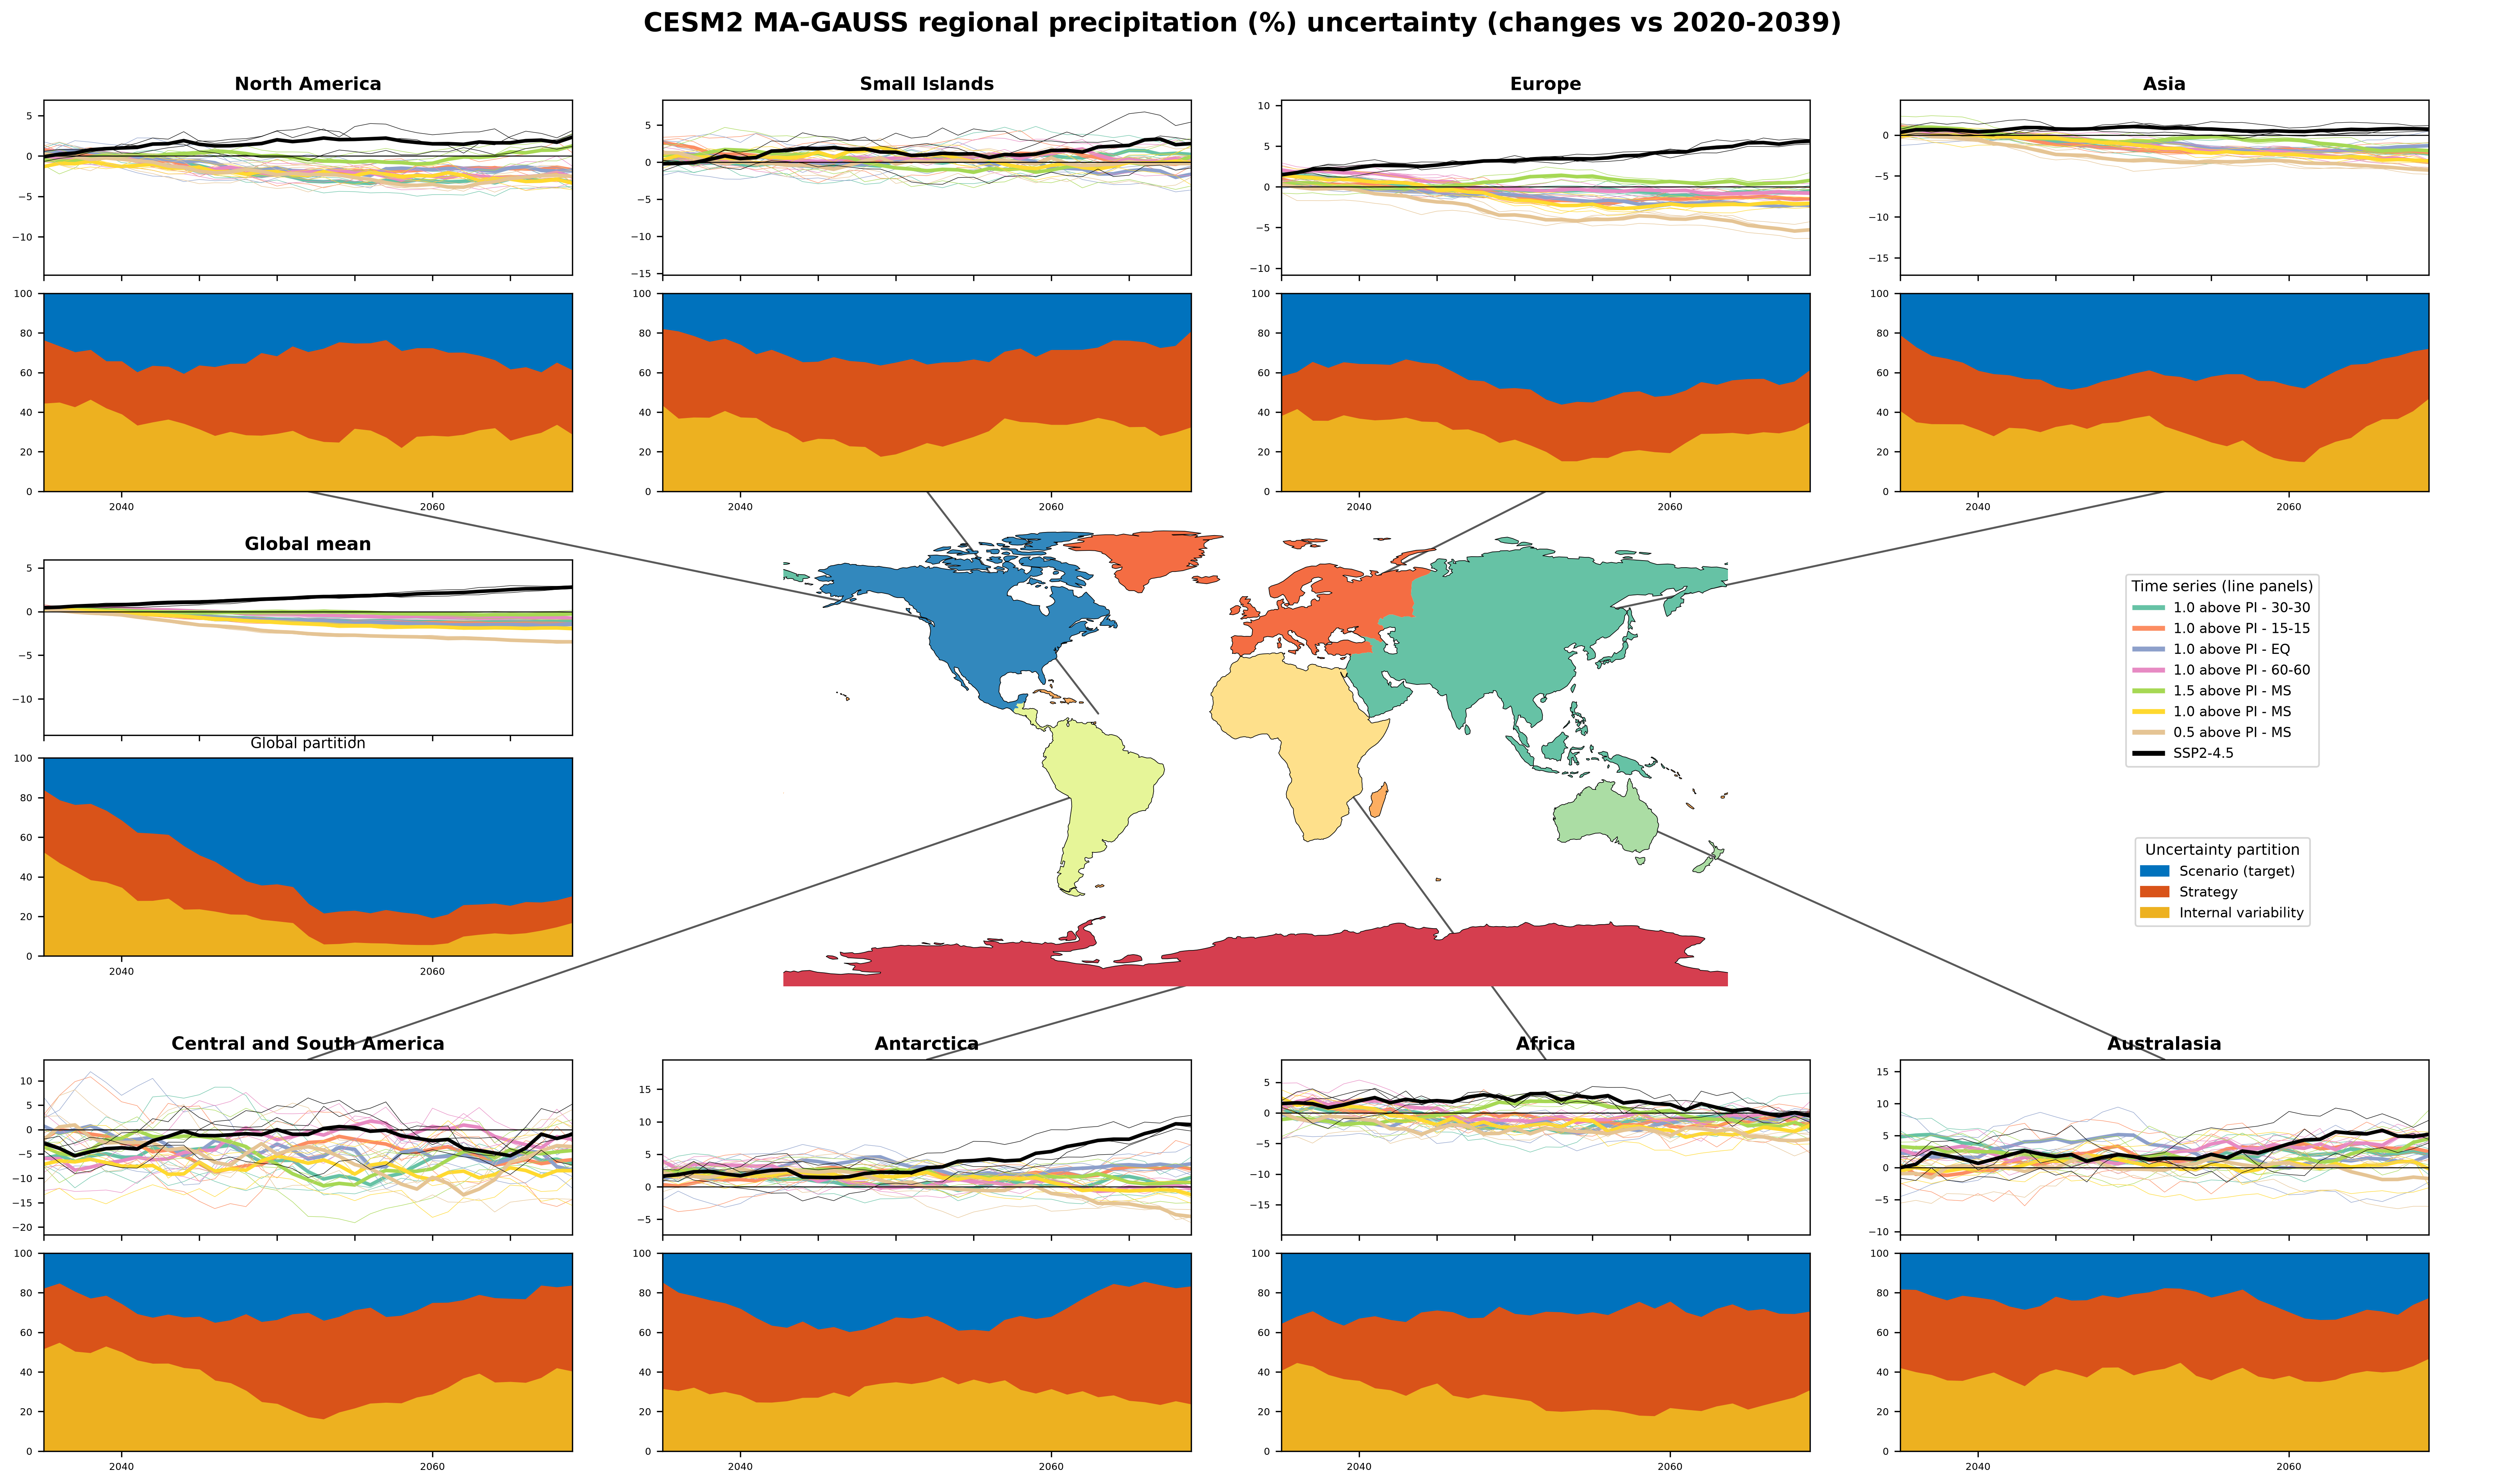
\includegraphics[width=0.95\linewidth]{figures/HS_plot_PRECT_regions_map.png}
\caption{As in Fig.~\ref{strategy_tas}, but for annual mean precipitation.}
\label{strategy_pr}
\end{figure*}

While not directly comparable, it is useful to mention alongside our results, the outcomes of the Precipitation Drivers and Responses MIP \citep[PDRMIP][]{PDRMIP2016} as an example of a model intercomparison effort trying to understand how various drivers of precipitation response differ across models. The substantial differences between the two protocols (namely, PDRMIP was focused on tropospheric increases of black carbon and SO$_4$, and had an increase, rather than a decrease, of global insolation), make it hard to do a like-for-like comparison, but in general it is worth noting that they found that tropical regions had a larger inter-model spread, and larger sensitivities to different drivers, compared to mid-latitudinal regions, which can help explain the results over Africa.

\section{Beyond our analyses: What isn't captured in these categories}

Our methodology has provided a first order quantification of the main uncertainty categories related to the climate modeling of SRM, using a wide range of SAI simulations. Clearly, analyses limited to climate model results will have the same limitations that the climate models themselves have at this point in time.

Nevertheless, there are several potentially important types of uncertainties that the framework described above cannot capture.
One example is the interaction between the land and oceanic carbon sinks and SRM. In the SSP CMIP6 scenarios used here, the concentrations of CO$_2$ and other gases are prescribed, and therefore are not directly affected by changes in the carbon cycles simulated by the land models. Previous research has shown that SRM would in fact enhance the carbon cycle \citep{Zhao2024}, both due to the combination of higher CO$_2$ concentrations and lower temperatures and due to the increase in diffuse radiation (a consequence of increased aerosol scattering), which is beneficial for net primary productivity, as it increases the amount of light that can reach the lower layers of the canopy. This potential increase in carbon sinks, which would in turn lead to lower CO$_2$ concentrations under any given SSP under an SRM scenario, is currently unaccounted for in CMIP6 models. On one hand, this leads to an easier separation of the effects of cooling and warming due to the aerosols, while on the other, it is an interaction that would affect the inter-model spread in different ways. Comparing CMIP7 models and scenarios, that will be emission rather than concentration driven \citep{ScenarioMIP}, with CMIP6 ones, will highlight the potential importance of this process.

Current Earth System modeling frameworks do not allow for a direct feedback between possible interventions, or changes in climate impacts, and emissions. This interaction could greatly increase the scenario uncertainty here discussed, considering both potential changes in emissions behavior due to the presence or perception of SAI and changes in economical choices related to emissions mitigation due to changes in risk profiles \citep[climate-society feedbacks, e.g.,][]{Beckage_2025}. Similarly, if one were to consider the willingness to deploy or not different strategies of SRM based on changes in risk or incentives, this could also affect the strategy and target space: depending on the design of the risk assessments, and on the methods used to understand these interactions (for instance, considering Integrated Assessment Models of different complexity versus models of the human-physical system), different conclusions could be reached about how the overall storyline uncertainty is affected.

%\subsection{Uncertainties, risks and confidence}

%Our definition of uncertainties as used in this work has a nuanced connection to the concept of ''risk'' when considering an SRM deployment that is worth being explicit about. Based on our results, we can say that, for instance, for the 6 GeoMIP models, modeling uncertainties in surface temperatures and precipitation changes under SAI are lower at both a global and regional level compared to climate change, in the sense that the modeled respons is more coherent across models in the former compared than the latter in a majority of the regions. However, such an assessment does not translate automatically to saying that SAI is, in itself, less ''risky'', even just from a climatic perspective.\\

%Following the IPCC definition of risk as ''the potential for adverse consequences'' resulting from ''dynamic interactions between climate-related hazards with the exposure and vulnerability of the affected human or ecological system to the hazards''  \citep[both definitions verbatim from][]{reisinger2020concept}, our analyses are only limited to looking at the potential climate drivers of hazards and furthermore, by looking at mean quantities, 

%\subsubsection{HEADING}



\conclusions  %% \conclusions[modified heading if necessary]

In this work, we have tried to provide a consistent framework for understanding and discussing uncertainties in Solar Radiation Modification modeling efforts. We have applied our efforts to a set of solar dimming and Stratospheric Aerosol Injection simulations, but our framework could be expanded to Marine Cloud Brightening or other methods as well. While there are many ways to envision uncertainty as a concept, in the context of those that can be explored through Earth System Modeling, our definition is simply that of a spread in projections at a global, regional and local level given under an envisioned SAI deployment.

We have shown that, when discussing the concept so defined, it is beneficial to expand the usual uncertainty framework considered for climate change simulations, consisting of scenario and inter-model uncertainty (together with internal variability), by separating the first into scenario (referring to the underlying GHG emissions trajectory), target (the purported aim of the SAI deployment), and strategy (the way in which that target can be achieved), whereas the second can be separated into inter-model climate uncertainty (how different models respond, given the same forcing) and inter-model SAI-specific uncertainty (how, given a specific target and strategy, do different models simulate the SAI deployment). This way, we can clarify the potential for further SAI-specific research to reduce such uncertainties, and separate that more specifically from the underlying climate modeling uncertainty, and we showed that, compared to climate change simulations, SAI-specific uncertainty is, in GeoMIP models, smaller and not larger than climate change uncertainty. In other terms, given a specific scenario, the inter-model spread is larger at any level (global, regional and local) if more warming is allowed to happen, compared to a case in which the warming is avoided through SAI.

The most important caveat of this work is that quantifying a result and its related uncertainty so defined is not the same as the confidence in the reliability of those results. Climate models are well tested and validated, but certainly do not lack shortcomings. Our analyses are based on the assumption that the sub-set of models used here are as reliable for climate change simulations as they are for SAI ones. We think that this is a reasonable conclusion - ultimately, projections of an Earth System that has less energy imbalance to respond to can be reasonably expected to diverge less \citep{MarMartin2015}.  Further study could show differently, for example, through an analogue of emergent constraints \citep[e.g.,][]{Hall2019}, which have been instrumental in validating climate models under climate change projections.

It is important to note that our analyses do not imply that this is the only way to quantify modeling uncertainty. Perturbed Parameter Ensembles (PPEs) are another important tool that can help understand how different parameterizations affect the results. But for none of the simulations we have analyzed here is there a PPE available (while some past ones exist), making it unfeasible to integrate them in our quantifications. If such a PPE existed, especially if focused on quantifying aerosol-uncertainty driven variance, it could provide another independent constraint on the $\sigma^2_{\mathrm{aerosols}}$ that we calculated here.\\

This leads us to outlining another challenge: to make better quantifications than ours, it would be very beneficial to have a consistent set up of simulations across model generations (i.e., CMIP5 to CMIP7). The problem is that, as Earth System Models evolve and improve, so does our understanding of potential SAI strategies, and our definitions of underlying climate scenarios (that is, there isn't an easy mapping between emission pathways between CMIP5, CMIP6 and CMIP7, so like-for-like comparisons are complicated). More recent GeoMIP simulations use different scenarios, strategies, and targets, following an evolved understanding from the community, but this, combined with the fact the sample of models used is different across GeoMIP generations, means that a precise assessment of how uncertainties evolve over time as models become more complex remains elusive. A more iterative process \citep[as proposed for instance by][]{visioni_living2024} in which the same scenarios are simulated with models once a new version is available, or after they have been improved following novel parameterizations or the integration of new observations, would allow for a more concrete quantification of how uncertainties in SAI evolve over time, and show how (and if) they can be reduced as new information comes in. 

To summarize this work, it is useful to think through an answer to the question ``Is the climate response to SAI uncertain?''. Granted that the answer one might be tempted to give is always ``It depends'' or ``Compared to what'', our analyses (combined with other results from the past and recent literature) suggest that some more specific yet correct answers could be as follows:

\begin{itemize}
    \item At the global level, there is full agreement between climate models that an increase in the stratospheric aerosol load would lead to reduced global mean temperatures due to a negative radiative forcing. There is uncertainty over how much increase in stratospheric aerosol load would be necessary given a specific cooling target (i.e., to cool by 1$^{\circ}$C globally), or how much SO$_2$ would be necessary to achieve such an increase. Such uncertainty arises from SAI-specific inter-model uncertainties and, partly, are also a function of the strategy uncertainty. When considering CO$_2$ emissions, and the interaction between emissions and concentrations, a part of the uncertainty can also arise from climate uncertainties related to the carbon cycle response.
    \item At the regional level, given a specific amount of cooling and and a specific injection strategy, there is uncertainty in both the temperature and precipitation regional response arising both from SAI-specific inter-model uncertainties (how the aerosols spread over the globe) and underlying inter-model climatic uncertainty (how the models respond to the same exact forcing). However, current modeling results suggest that, in the same set of models, inter-model uncertainty in response to a specific amount of warming is on average larger for both temperature and precipitation in a scenario in which global warming increases, compared to a scenario in which such global warming is prevented with SAI. This assumes an equal confidence in the climate models' responses to a GHG forcing and to a stratospheric aerosol forcing.
    \item The uncertainties in the modeled regional responses to SAI also depend on the overall chosen target (how much cooling) and strategy (how to achieve that cooling). For a comprehensive set of different strategies that aim to cool both hemispheres with some symmetry, the regional temperature response is mainly driven by decisions over the global cooling target, whereas the regional precipitation responses in most regions are equally driven by the details of the strategy chosen.
\end{itemize}

Overall, these three points underscore the importance of clarifying exactly which source of uncertainty one is thinking of when discussing them in the context of SAI, especially as it pertains to reducing them. It is likely that inter-model climate uncertainties can be reduced through the same mechanisms that would reduce inter-model uncertainties pertaining to global warming projections (higher horizontal resolution, better parameterizations, better mechanistic understanding, and resolution of underlying regional climate processes), whereas inter-model SAI uncertainties may be reducible through research that better resolves stratospheric processes, from nucleation of particles to large-scale transport to stratosphere-troposphere coupling given a stratospheric perturbation. On the other hand, scenario, target and strategy uncertainties belong to a much fuzzier - but not less important - domain, in which ``more research'' is not necessarily going to constrain them in the future. Partly, they can be constrained by focusing on plausible scenarios (which is the most likely paths that emissions and carbon removal will take in the future), plausible cooling targets (considering the low likelihood and lack of desirability of too large, abrupt cooling amounts) and plausible intervention strategies (potentially constraining them through economic analyses of regional and local benefits, as well as through analyses of the actual size of meaningfully different strategies from a climatic perspective). However, human behavior cannot be constrained solely through optimization analyses, and it remains critical that different methods of study and analyses are welcomed in trying to think through future scenarios that include SAI. 

Concluding, it is very important to underscore that our results should not be read as a simplistic claim that SAI is not uncertain, or that what we have presented is sufficient to make decisions about SAI deployment. Quite the contrary, they highlight the specific challenge that is posed by SAI as a concept and to SAI as a research field: the addition of a further dimension, or rather a set of dimensions, on top of what is already a complicated human, economic and natural system. It is certainly likely that the reduction in climatic uncertainty that is in theory attainable through a uniform, well done deployment might be matched, if not dwarfed, by the added uncertainty to the socio-political realm, of whether such a well-envisioned deployment is tenable at all.

Ultimately, however, our results do make the point that picturing the climatic response to SAI as inherently ``unknowable'' is not supported by modeling results, and that further improvements to our understanding of the many physical processes involved in stratospheric aerosol can further build confidence in what such a response would be.

%% The following commands are for the statements about the availability of data sets and/or software code corresponding to the manuscript.
%% It is strongly recommended to make use of these sections in case data sets and/or software code have been part of your research the article is based on.

\codeavailability{TEXT} %% use this section when having only software code available


\dataavailability{TEXT} %% use this section when having only data sets available


\codedataavailability{TEXT} %% use this section when having data sets and software code available


\sampleavailability{TEXT} %% use this section when having geoscientific samples available


\videosupplement{TEXT} %% use this section when having video supplements available


\appendix
\section{}    %% Appendix A

\subsection{}     %% Appendix A1, A2, etc.


\noappendix       %% use this to mark the end of the appendix section. Otherwise the figures might be numbered incorrectly (e.g. 10 instead of 1).

%% Regarding figures and tables in appendices, the following two options are possible depending on your general handling of figures and tables in the manuscript environment:

%% Option 1: If you sorted all figures and tables into the sections of the text, please also sort the appendix figures and appendix tables into the respective appendix sections.
%% They will be correctly named automatically.

%% Option 2: If you put all figures after the reference list, please insert appendix tables and figures after the normal tables and figures.
%% To rename them correctly to A1, A2, etc., please add the following commands in front of them:

\appendixfigures  %% needs to be added in front of appendix figures

\appendixtables   %% needs to be added in front of appendix tables

%% Please add \clearpage between each table and/or figure. Further guidelines on figures and tables can be found below.



\authorcontribution{TEXT} %% this section is mandatory

\competinginterests{TEXT} %% this section is mandatory even if you declare that no competing interests are present

\disclaimer{TEXT} %% optional section

\begin{acknowledgements}
Support for BK was provided in part by NOAA's Climate Program Office, Earth’s Radiation Budget (ERB) (Grant NA22OAR4310479), and the Indiana University Environmental Resilience Institute. SV and TS received funding from the Karbacher Fonds, Graub\"unden, Switzerland and from the Simons Fundation (grant Nr. SFI-MPS-SRM-00005217 and SFI-MPS-SRM-00005208).
\end{acknowledgements}




%% REFERENCES

%% The reference list is compiled as follows:

%% Since the Copernicus LaTeX package includes the BibTeX style file copernicus.bst,
%% authors experienced with BibTeX only have to include the following two lines:
%%
\bibliographystyle{copernicus}
\bibliography{reference.bib}
%%
%% URLs and DOIs can be entered in your BibTeX file as:
%%
%% URL = {http://www.xyz.org/~jones/idx_g.htm}
%% DOI = {10.5194/xyz}


%% LITERATURE CITATIONS
%%
%% command                        & example result
%% \citet{jones90}|               & Jones et al. (1990)
%% \citep{jones90}|               & (Jones et al., 1990)
%% \citep{jones90,jones93}|       & (Jones et al., 1990, 1993)
%% \citep[p.~32]{jones90}|        & (Jones et al., 1990, p.~32)
%% \citep[e.g.,][]{jones90}|      & (e.g., Jones et al., 1990)
%% \citep[e.g.,][p.~32]{jones90}| & (e.g., Jones et al., 1990, p.~32)
%% \citeauthor{jones90}|          & Jones et al.
%% \citeyear{jones90}|            & 1990



%% FIGURES

%% When figures and tables are placed at the end of the MS (article in one-column style), please add \clearpage
%% between bibliography and first table and/or figure as well as between each table and/or figure.

% The figure files should be labelled correctly with Arabic numerals (e.g. fig01.jpg, fig02.png).


%% ONE-COLUMN FIGURES

%%f
%\begin{figure}[t]
%\includegraphics[width=8.3cm]{FILE NAME}
%\caption{TEXT}
%\end{figure}
%
%%% TWO-COLUMN FIGURES
%
%%f
%\begin{figure*}[t]
%\includegraphics[width=12cm]{FILE NAME}
%\caption{TEXT}
%\end{figure*}
%
%
%%% TABLES
%%%
%%% The different columns must be seperated with a & command and should
%%% end with \\ to identify the column brake.
%
%%% ONE-COLUMN TABLE
%
%%t
%\begin{table}[t]
%\caption{TEXT}
%\begin{tabular}{column = lcr}
%\tophline
%
%\middlehline
%
%\bottomhline
%\end{tabular}
%\belowtable{} % Table Footnotes
%\end{table}
%
%%% TWO-COLUMN TABLE
%
%%t
%\begin{table*}[t]
%\caption{TEXT}
%\begin{tabular}{column = lcr}
%\tophline
%
%\middlehline
%
%\bottomhline
%\end{tabular}
%\belowtable{} % Table Footnotes
%\end{table*}
%
%%% LANDSCAPE TABLE
%
%%t
%\begin{sidewaystable*}[t]
%\caption{TEXT}
%\begin{tabular}{column = lcr}
%\tophline
%
%\middlehline
%
%\bottomhline
%\end{tabular}
%\belowtable{} % Table Footnotes
%\end{sidewaystable*}
%
%
%%% MATHEMATICAL EXPRESSIONS
%
%%% All papers typeset by Copernicus Publications follow the math typesetting regulations
%%% given by the IUPAC Green Book (IUPAC: Quantities, Units and Symbols in Physical Chemistry,
%%% 2nd Edn., Blackwell Science, available at: http://old.iupac.org/publications/books/gbook/green_book_2ed.pdf, 1993).
%%%
%%% Physical quantities/variables are typeset in italic font (t for time, T for Temperature)
%%% Indices which are not defined are typeset in italic font (x, y, z, a, b, c)
%%% Items/objects which are defined are typeset in roman font (Car A, Car B)
%%% Descriptions/specifications which are defined by itself are typeset in roman font (abs, rel, ref, tot, net, ice)
%%% Abbreviations from 2 letters are typeset in roman font (RH, LAI)
%%% Vectors are identified in bold italic font using \vec{x}
%%% Matrices are identified in bold roman font
%%% Multiplication signs are typeset using the LaTeX commands \times (for vector products, grids, and exponential notations) or \cdot
%%% The character * should not be applied as mutliplication sign
%
%
%%% EQUATIONS
%
%%% Single-row equation
%
%\begin{equation}
%
%\end{equation}
%
%%% Multiline equation
%
%\begin{align}
%& 3 + 5 = 8\\
%& 3 + 5 = 8\\
%& 3 + 5 = 8
%\end{align}
%
%
%%% MATRICES
%
%\begin{matrix}
%x & y & z\\
%x & y & z\\
%x & y & z\\
%\end{matrix}
%
%
%%% ALGORITHM
%
%\begin{algorithm}
%\caption{...}
%\label{a1}
%\begin{algorithmic}
%...
%\end{algorithmic}
%\end{algorithm}
%
%
%%% CHEMICAL FORMULAS AND REACTIONS
%
%%% For formulas embedded in the text, please use \chem{}
%
%%% The reaction environment creates labels including the letter R, i.e. (R1), (R2), etc.
%
%\begin{reaction}
%%% \rightarrow should be used for normal (one-way) chemical reactions
%%% \rightleftharpoons should be used for equilibria
%%% \leftrightarrow should be used for resonance structures
%\end{reaction}
%
%
%%% PHYSICAL UNITS
%%%
%%% Please use \unit{} and apply the exponential notation


\end{document}
